\chapter{Laboratorio 3: \\Clock gating, pipelining and parallelizing}
Durante questa esperienza di laboratorio verranno analizzate una serie di tecniche per ridurre i consumi mediante l'ottimizzazione dell'architettura dei circuiti.
\section{A first approach to clock gating}
Un prima tecnica utilizzata per ridurre i consumi andando a lavorare sull'architettura è il \textit{Clock Gating}. Questa tecnica permette di "staccare" il clock ad un determinato blocco del mio circuito, quando questo non deve lavorare. Un circuito di massima è riportato in Figura \ref{clock_gating}. \\
\begin{figure}[!htb]
	\centering
	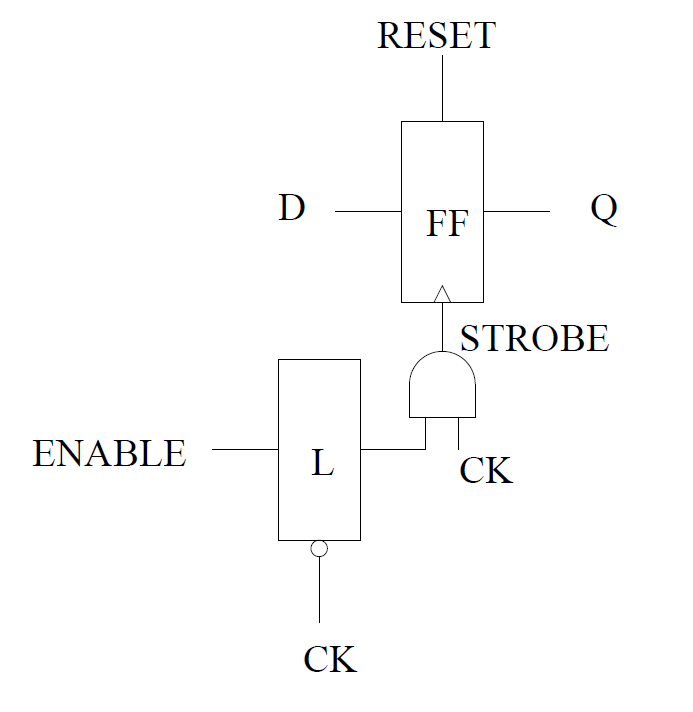
\includegraphics[scale=0.60]{immagini/clock_gating}
	\caption{\textit{Schema implementativo della tecnica del Clock Gating}}
	\label{clock_gating}
\end{figure}
\newpage
\noindent Nella prima parte dell'esperienza viene chiesto di analizzare il file \textit{ckgbug.vhd} che contiene la descrizione VHDL di una struttura composta da due registri in cascata, denominati L1 ed L2. La tecnica del clock gating viene applicata al secondo registro, mediante una AND tra il clock e un segnale di ENABLE. \\
Bisogna prestare attenzione al fatto che i segnali di ingresso dei due registri (D1 e D2) siano rispettivamente \textit{std\_logic\_vector (7 downto 0)} e \textit{std\_logic\_vector (0 to 7)}. \\
In una prima simulazione, si forza il segnale D1 al valore '01111111' e, attivando il segnale di ENABLE, ci si aspetterebbe che D2, al colpo di clock successivo, vada al valore '111111110' e che l'uscita di L2, denominata D3, vada al valore '01111111' al colpo di clock ancora successivo. In realtà la simulazione porta al risultato in Figura \ref{clock_gat1}.
\begin{figure}[!htb]
	\centering
	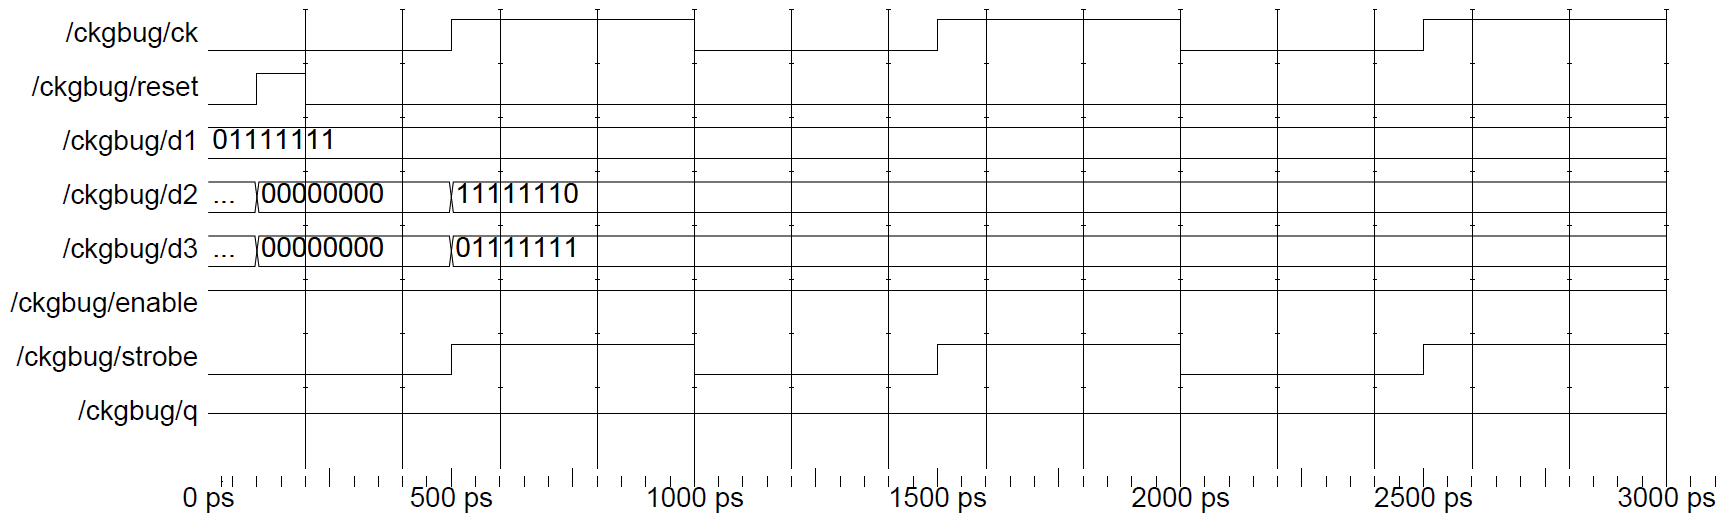
\includegraphics[scale=0.6]{immagini/clock_gating1}
	\caption{\textit{Timing simulazione}}
	\label{clock_gat1}
\end{figure}
Si può ben notare come l'uscita D3 dopi esattamente D1 dopo un solo colpo di clock. Questo è dovuto al fatto che il clock gated arriva a L2 un "passo di simulazione" dopo L1, perchè il simulatore programma il calcolo dell'uscita AND dopo l'assegnazione del clock. Quindi accade come se l'AND avesse un ritardo interno. \\
La traccia suggerisce che si può risolvere questo inconveniente andando ad aggiungere un ritardo \textit{Clock-to-Output} pari a 0.1 ps all'uscita del generico Flip-Flop. Andando a risimulare il file, si ottiene il comportamento desiderato, che viene riportato in Figura \ref{clock_gat2}. \\
\newpage
\begin{figure}[!htb]
	\centering
	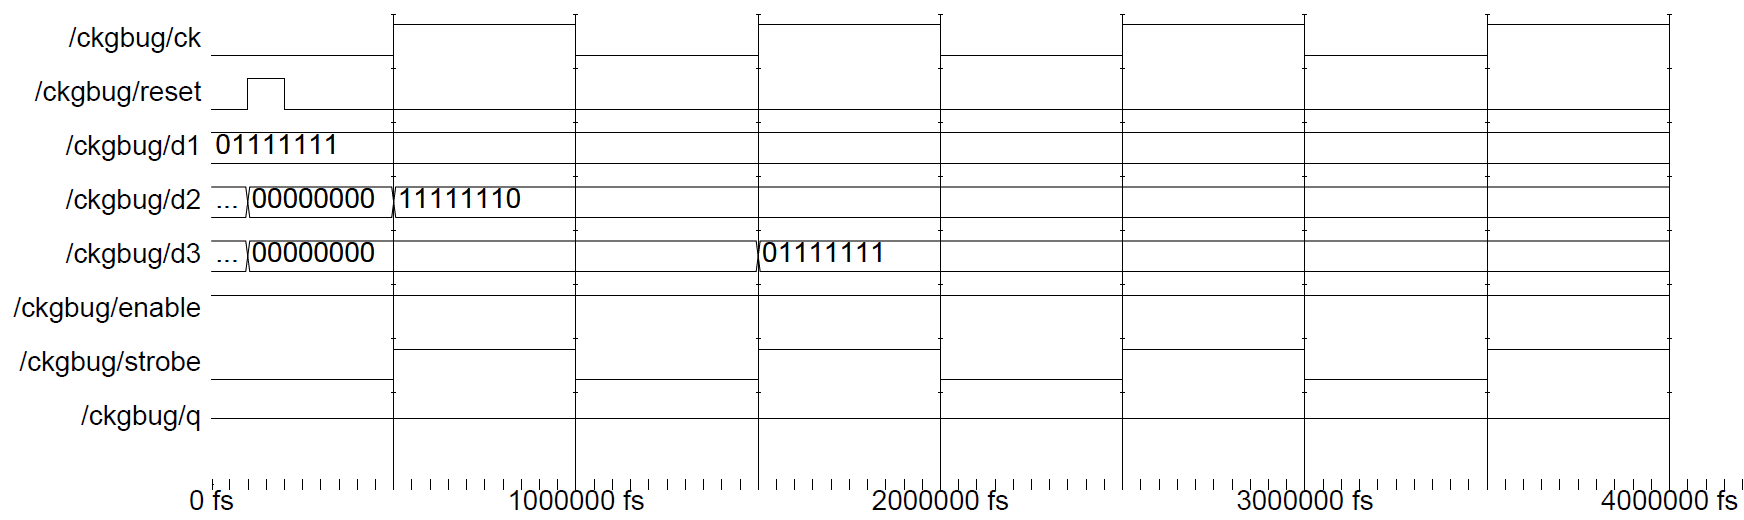
\includegraphics[scale=0.6]{immagini/clock_gating2}
	\caption{\textit{Timing simulazione con ritardo clk-to-out=0.1ps}}
	\label{clock_gat2}
\end{figure}
\noindent Infine si aggiunge un ulteriore ritardo alla porta AND pari a 0.2 ps, ossia un tempo superiore a quello \textit{Clock-to-Output} inserito in precendenza. In questo modo si va a violare il $t_{hold}$ e dunque il circuito ritorna nella situazione precedente con un funzionamento non corretto. Il risultato della simulazione è riportato in Figura \ref{clock_gat3}. \\
\begin{figure}[!htb]
	\centering
	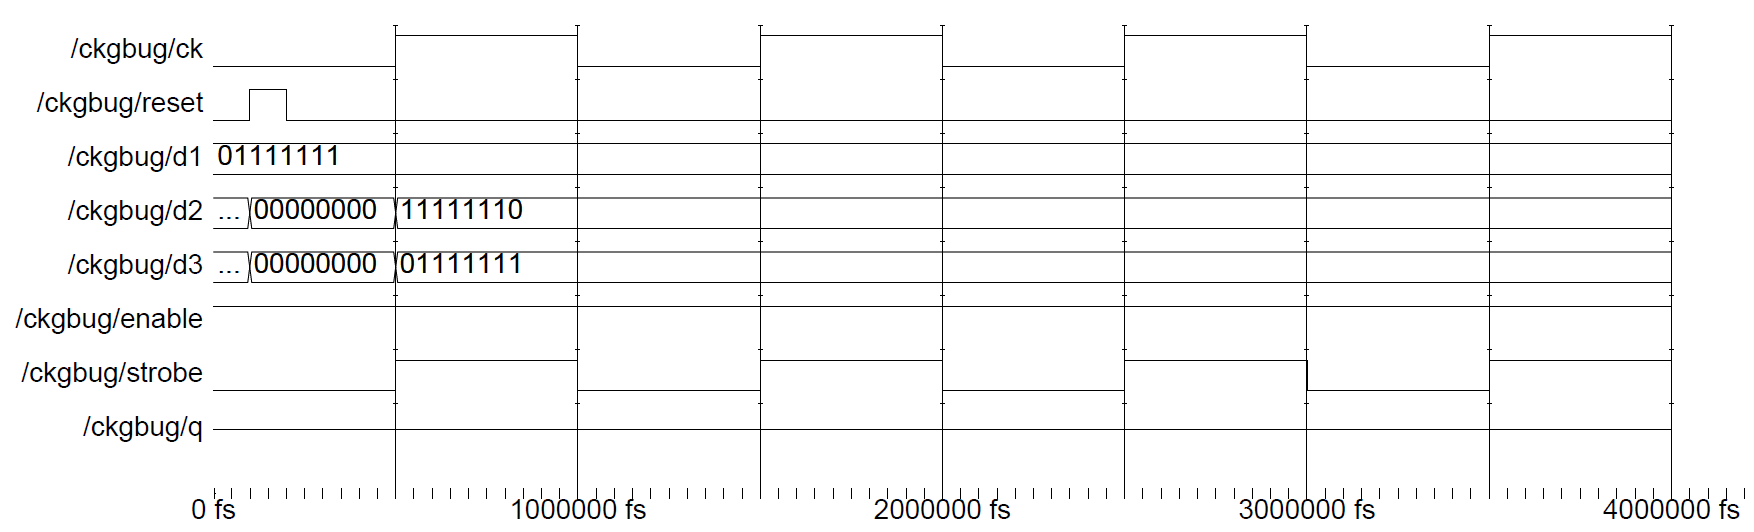
\includegraphics[scale=0.6]{immagini/clock_gating3}
	\caption{\textit{Timing simulazione, ritardo AND di 0.2ps}}
	\label{clock_gat3}
\end{figure}
\newpage
\section{Clock Gating for a complex circuit}
Nella seguente sezione viene chiesto di analizzare il funzionamento e in seguito il consumo di potenza, applicando il concetto del clock gating, nel circuito illustrato in Figura \ref{circuito_3_2}.\\
\begin{figure}[!htb]
	\centering
	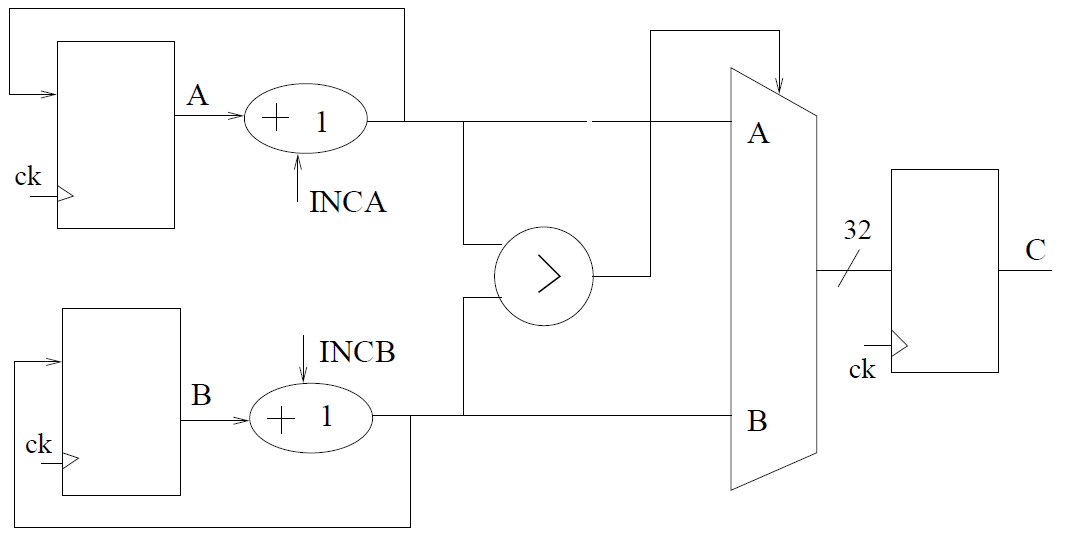
\includegraphics[scale=0.8]{immagini/circuito_3_2}
	\caption{\textit{Schema circuito}}
	\label{circuito_3_2}
\end{figure}
\\
Si prova, esclusivamente a livello cartaceo ad applicare la tecnica del Clock Gating al circuito in figura, ottenendo il circuito in Figura \ref{clkgating}.\\
\begin{figure}[!htb]
	\centering
	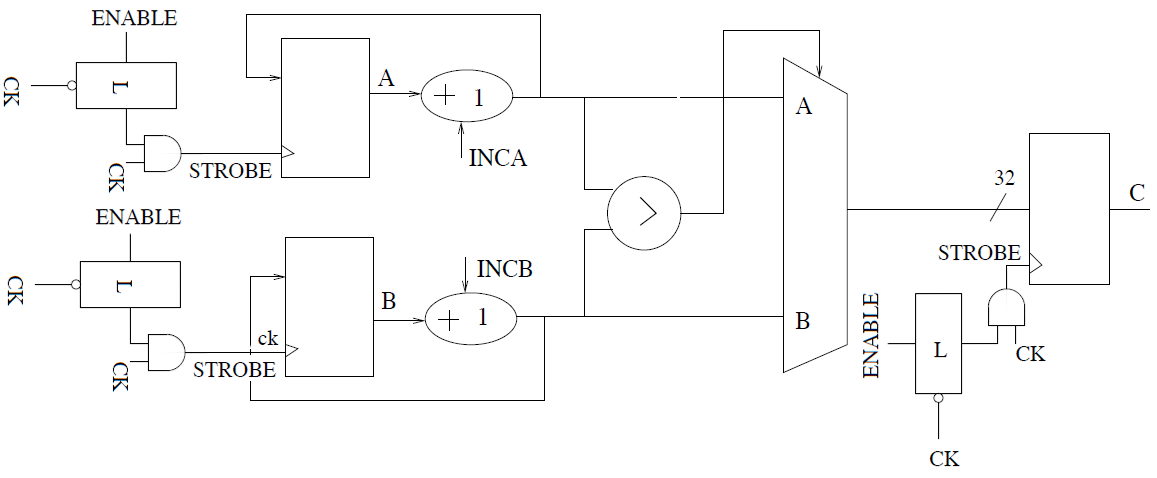
\includegraphics[scale=0.3]{immagini/clkgating}
	\caption{\textit{Schema circuito con clock gating}}
	\label{clkgating}
\end{figure}
\\
Si è proceduto dunque alla sintesi del circuito, sempre tramite \textit{Synopsis}, creando un clock con periodo pari a 5 s. Tramite il comando \textit{report\_power -include\_input\_nets} si è potuto ricavare un resoconto dei contributi di potenza dissipata, che vengono riportati in Figura \ref{3_1}. \\
\begin{figure}[!htb]
	\centering
	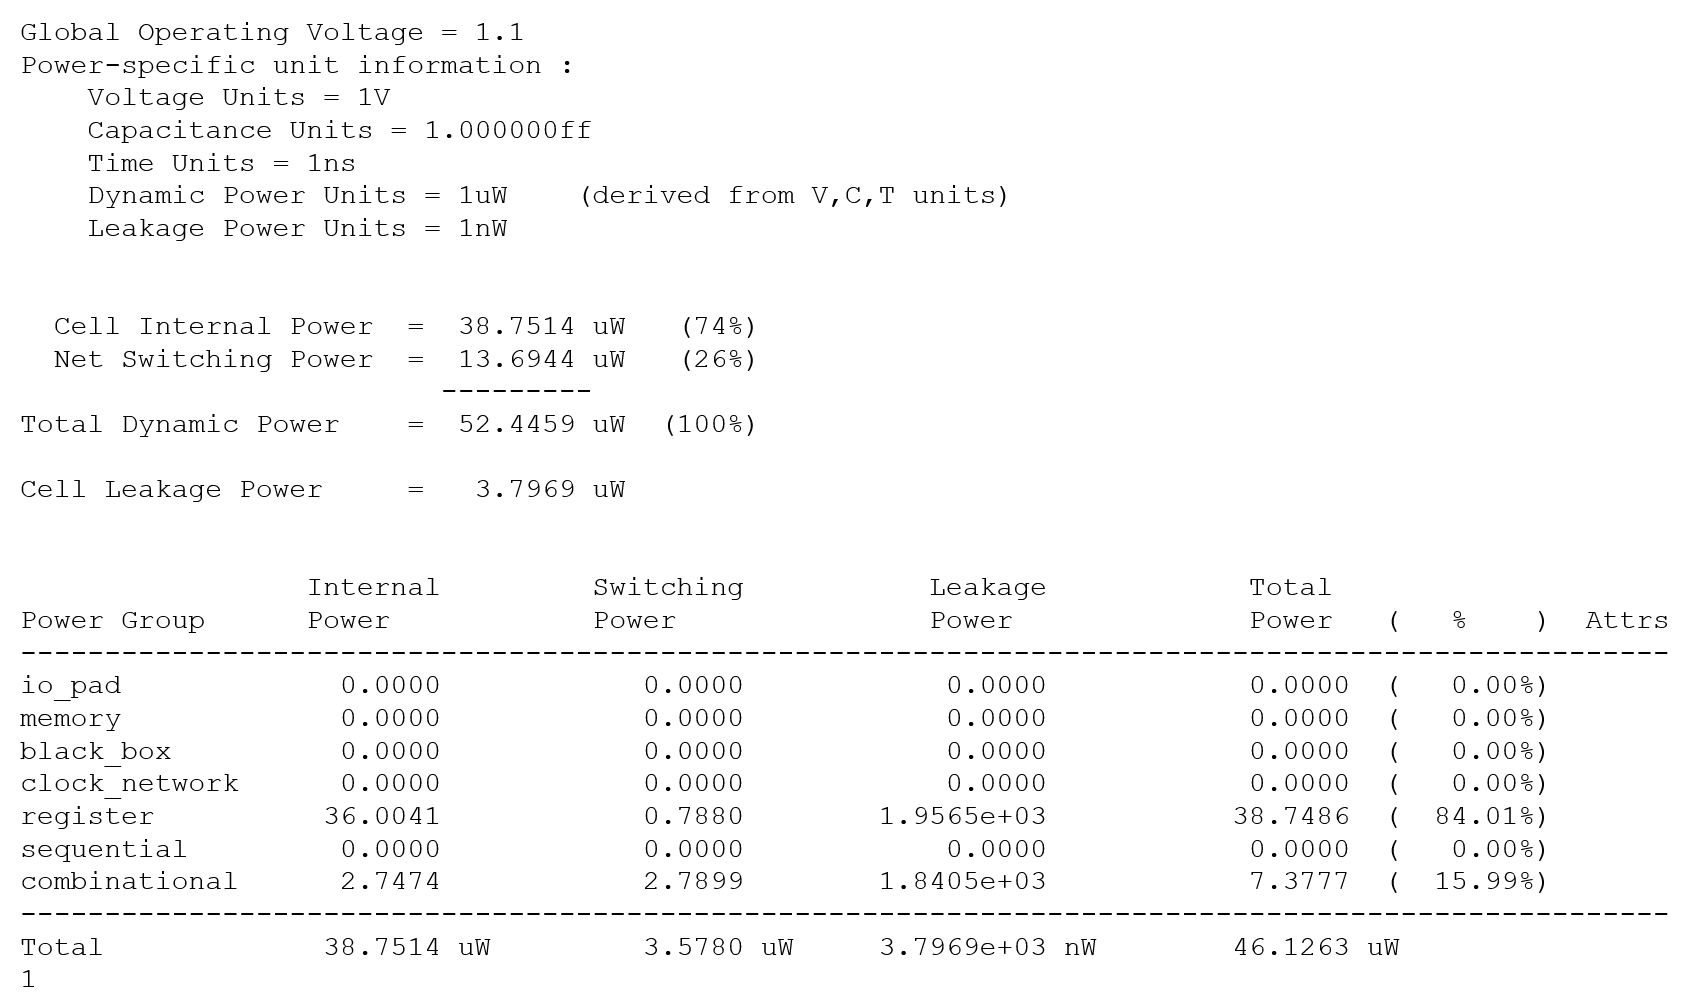
\includegraphics[scale=0.7]{immagini/3_1}
	\caption{\textit{Power report nets}}
	\label{3_1}
\end{figure}
\\
Si è poi andato ad eseguire un'analisi più dettagliata dei contributi tramite il comando \textit{report\_power -net -include\_input\_nets}, che viene riportato in Figura \ref{3_2}. \\
\begin{figure}[!htb]
	\centering
	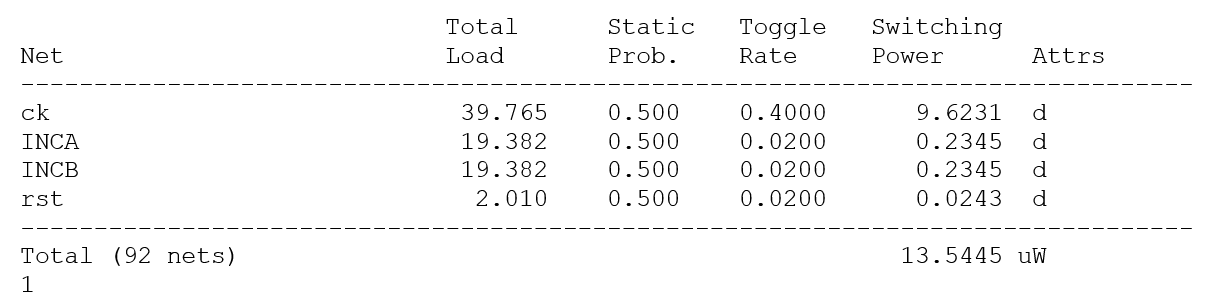
\includegraphics[scale=0.9]{immagini/3_2}
	\caption{\textit{Power report input nets}}
	\label{3_2}
\end{figure}
\\
Come si può ben notare dalla quarta colonna, il toogle rate dei vari ingressi presenta una \textit{static probability} pari a 0.5, che non risulta essere un valore sempre ragionevole. \\
Questo valore viene assegnato di default dal software, che però, tramite degli appositi comandi, permette di settare valori diversi di Toogle Rate a determinati segnali. Si è allora modificato il toggle rate del clock e del reset portandoli rispettivamente a 2 e a 0. Queste modifiche portano ad un risparmio di potenza del 20\% rispetto al caso precedente. Il report di potenza risultante viene raffigurato in Figura \ref{3_3}.
\begin{figure}[!htb]
	\centering
	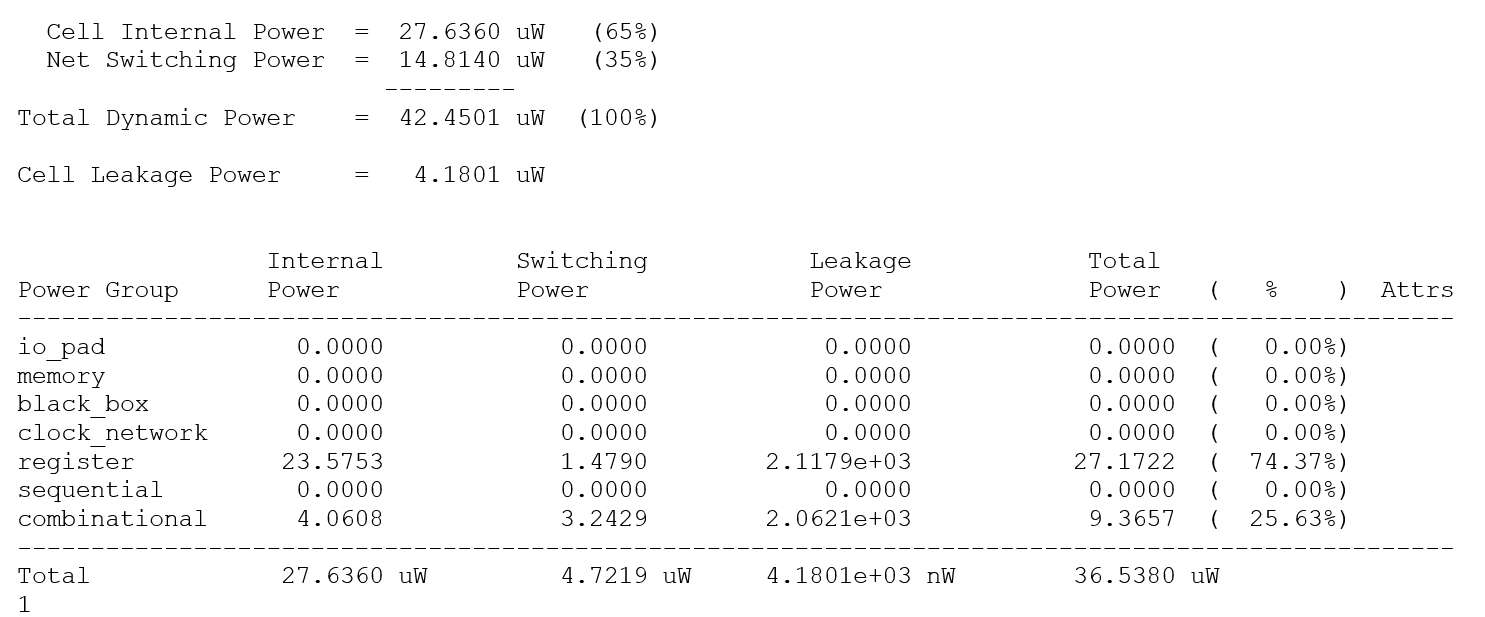
\includegraphics[scale=0.8]{immagini/3_3}
	\caption{\textit{Power report con toggle del clock pari a 2}}
	\label{3_3}
\end{figure}
Si va ora a modificare anche la probabilità degli input, portando sia INCA che INCB ad un Toggle Rate pari a 0.12. Si ottiene allora un risparmio ulteriore di potenza, come testimoniato da Power Report riportati in Figura \ref{3_4} e \ref{3_5}.
\begin{figure}[!htb]
	\centering
	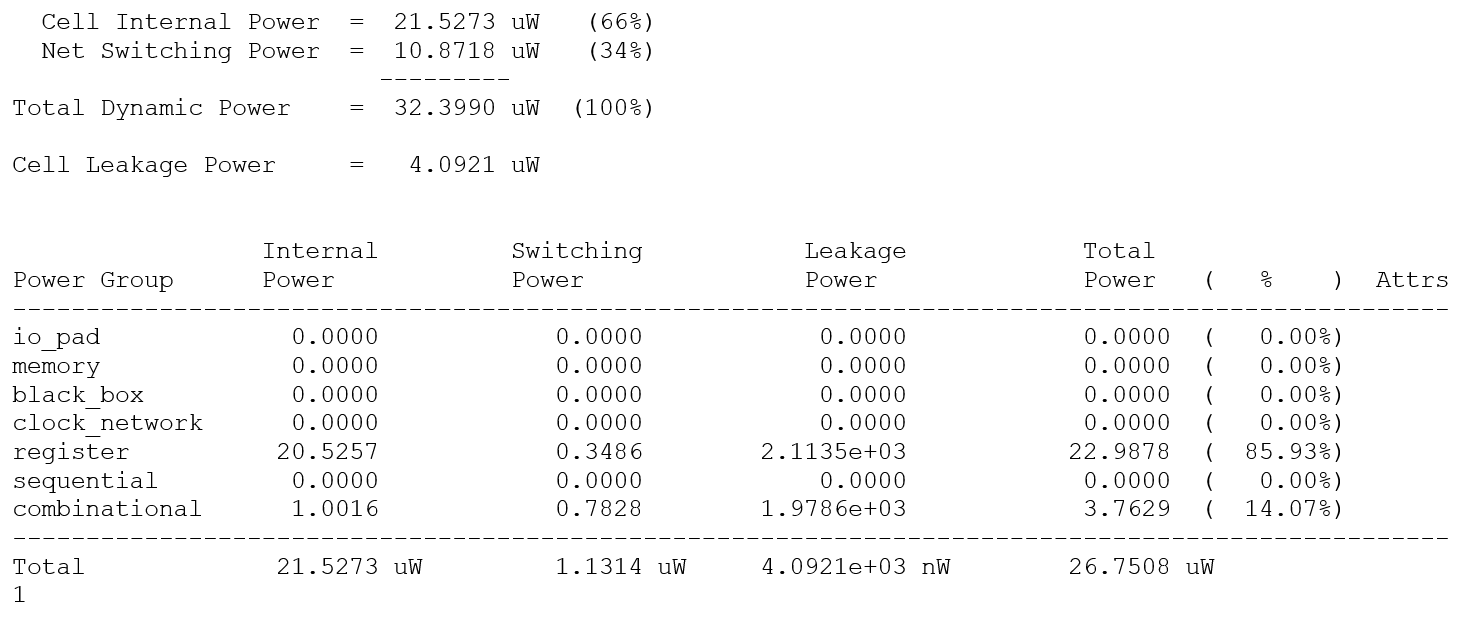
\includegraphics[scale=0.8]{immagini/3_4}
	\caption{\textit{Power report con toggle rate pari a 0.12}}
	\label{3_4}
\end{figure}
\begin{figure}[!htb]
	\centering
	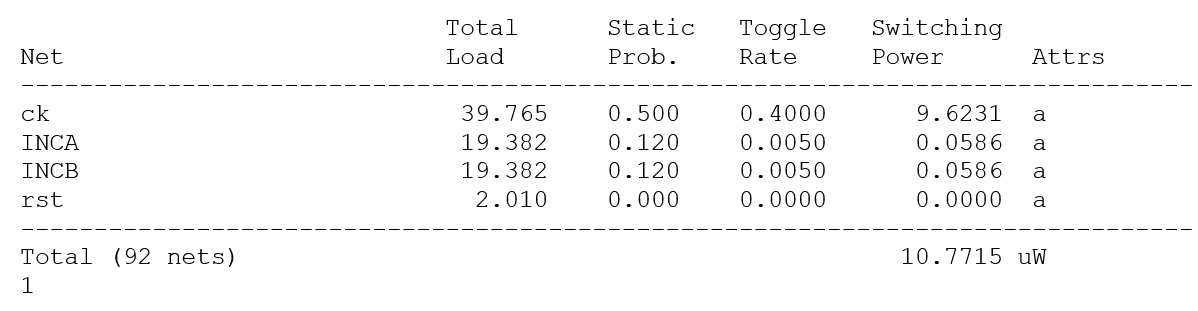
\includegraphics[scale=0.9]{immagini/3_5}
	\caption{\textit{Power report input nets}}
	\label{3_5}
\end{figure}
\newpage
\noindent Infine, tramite il comando \textit{report cell}, si riesce ad ottenere il numero di celle impiegate con la relativa dimensione. Viene riportato in Figura \ref{3_6}. Si può ben notare come nel caso analizzato le celle siano 74 e l'area utilizzata sia $229.292007 \mu m^{2}$ \\
\begin{figure}[!htb]
	\centering
	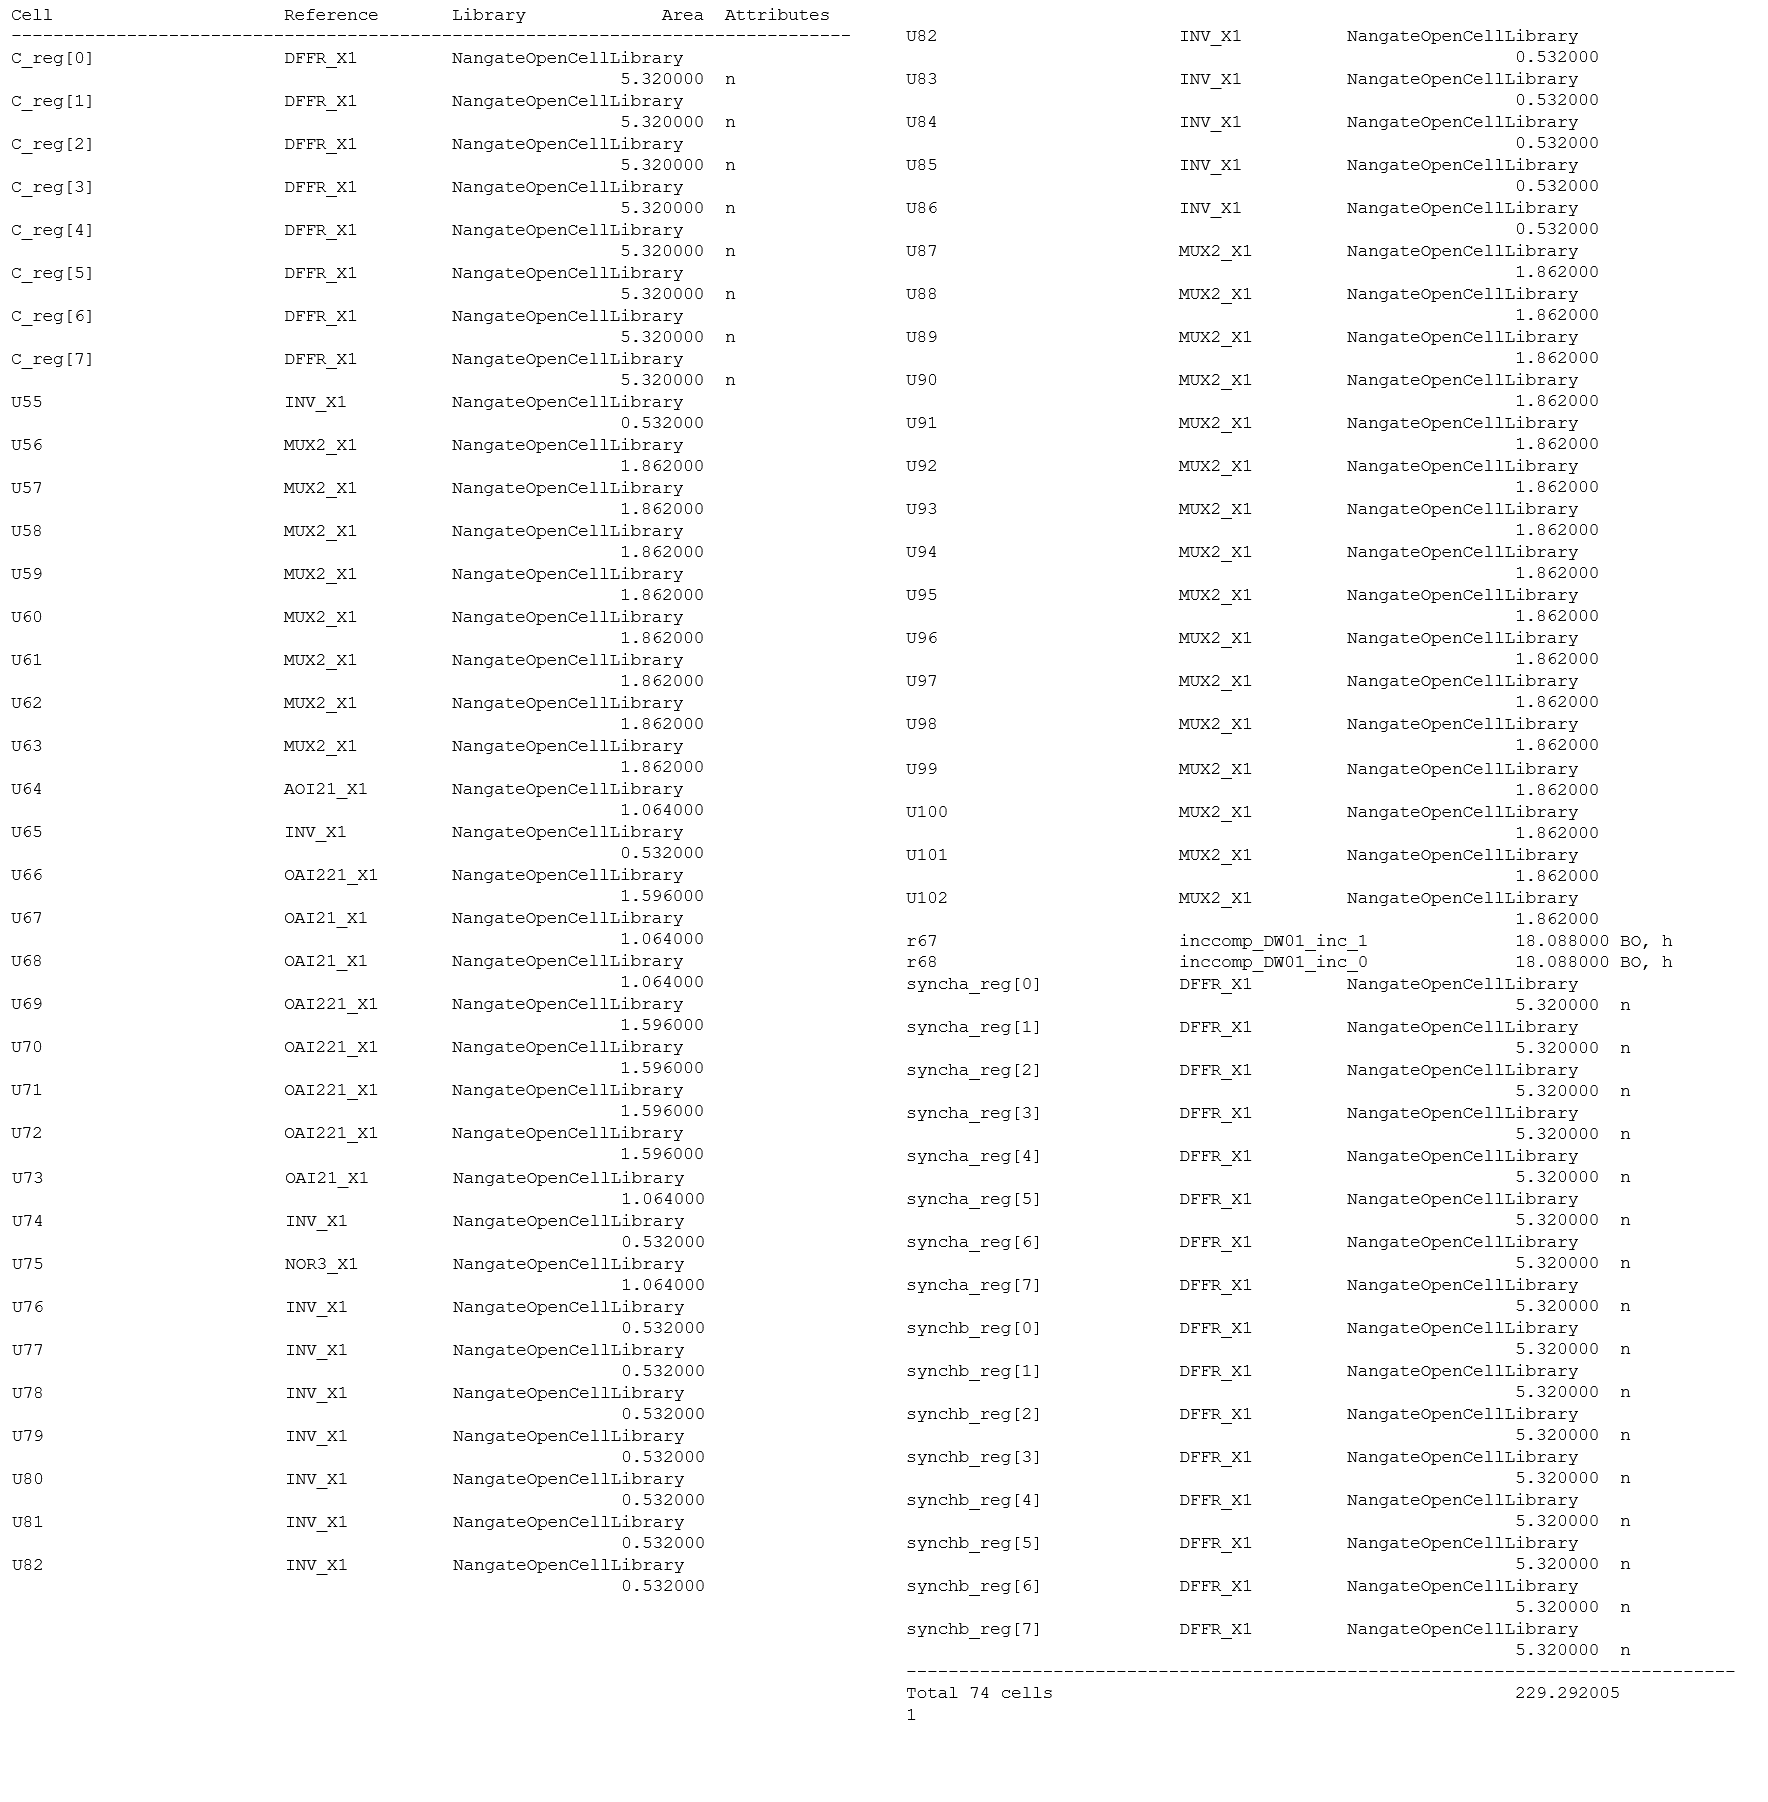
\includegraphics[scale=0.65]{immagini/3_6}
	\caption{\textit{Report cell}}
	\label{3_6}
\end{figure}
\newpage
Ora si ri-eseguono le medesime simulazioni, ma utilizzando il circuito dove è stato applicata la tecnica del Clock Gating. Inizialmente si sono lasciati tutti i parametri esattamente come la prima analisi, quindi tutte le probabilità pari a 0.5, e si è ottenuto comunque una potenza inferiore del 16\% rispetto al caso senza la tecnica del Clock Gating. Il tutto viene riportato in Figura \ref{3_7} e \ref{3_8}. \\
\begin{figure}[!htb]
	\centering
	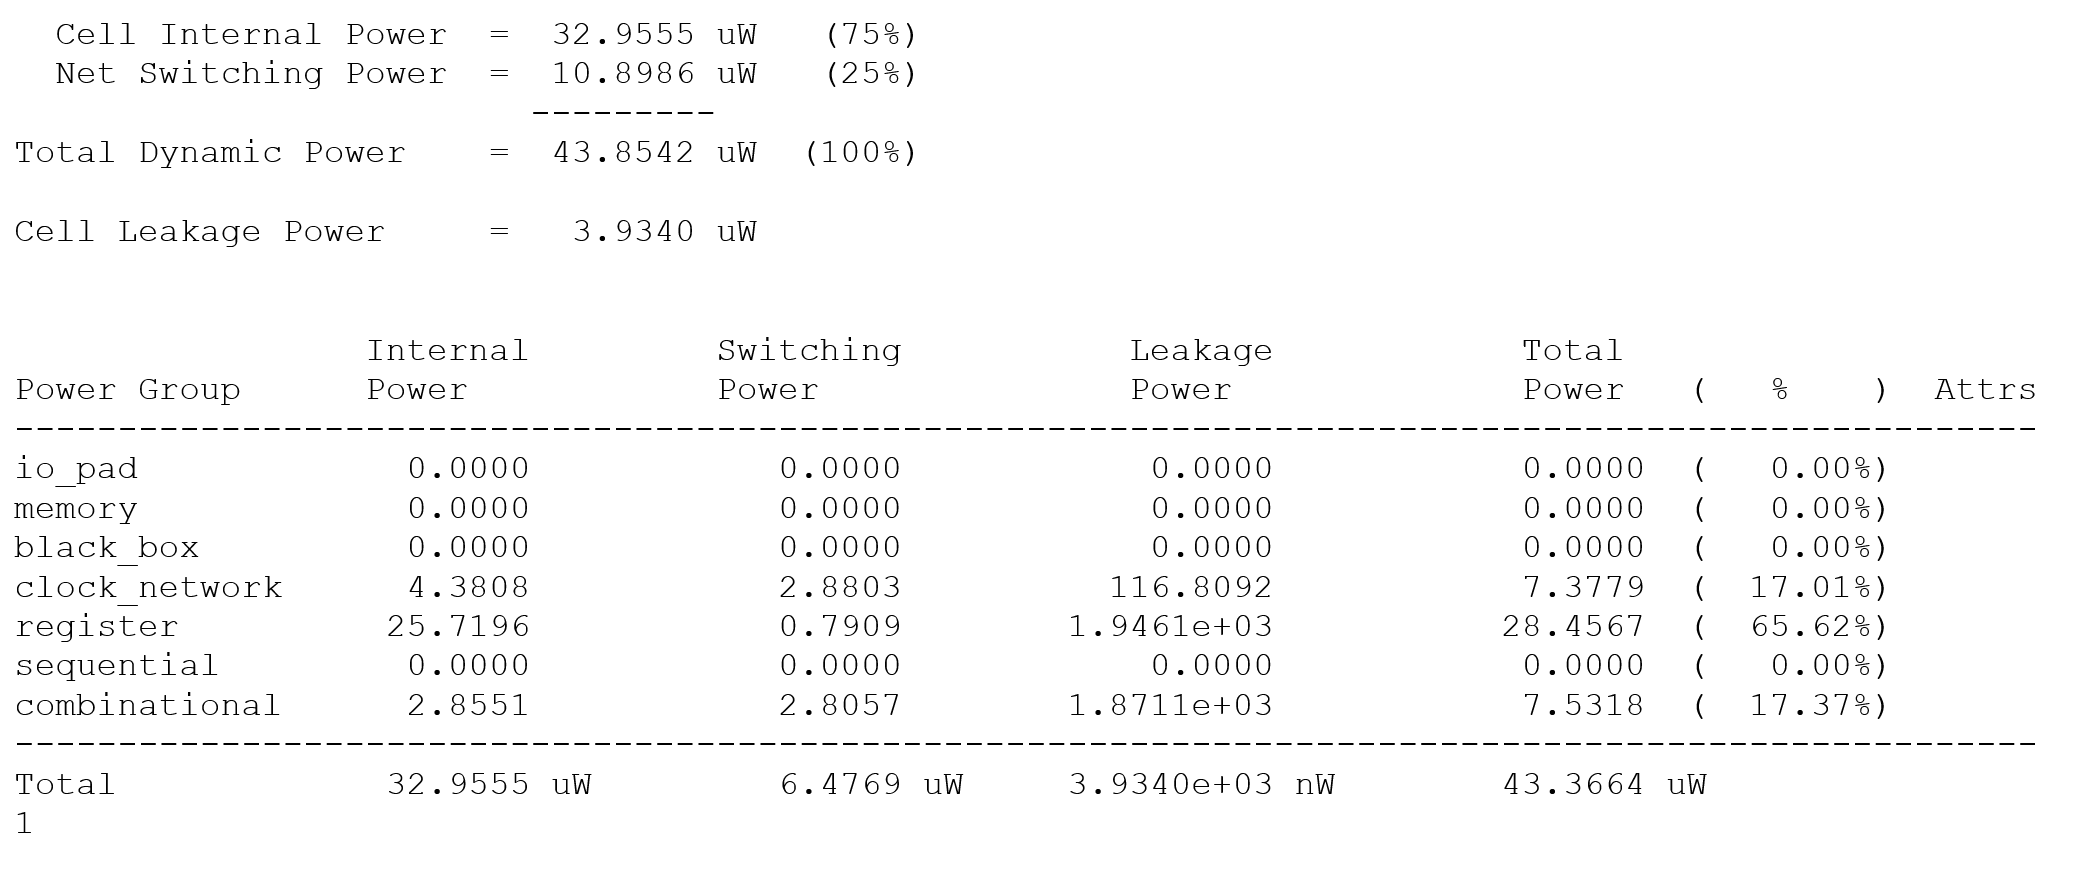
\includegraphics[scale=0.5]{immagini/3_7}
	\caption{\textit{Power report circuito con clock gating e condizioni iniziali}}
	\label{3_7}
\end{figure}
\begin{figure}[!htb]
	\centering
	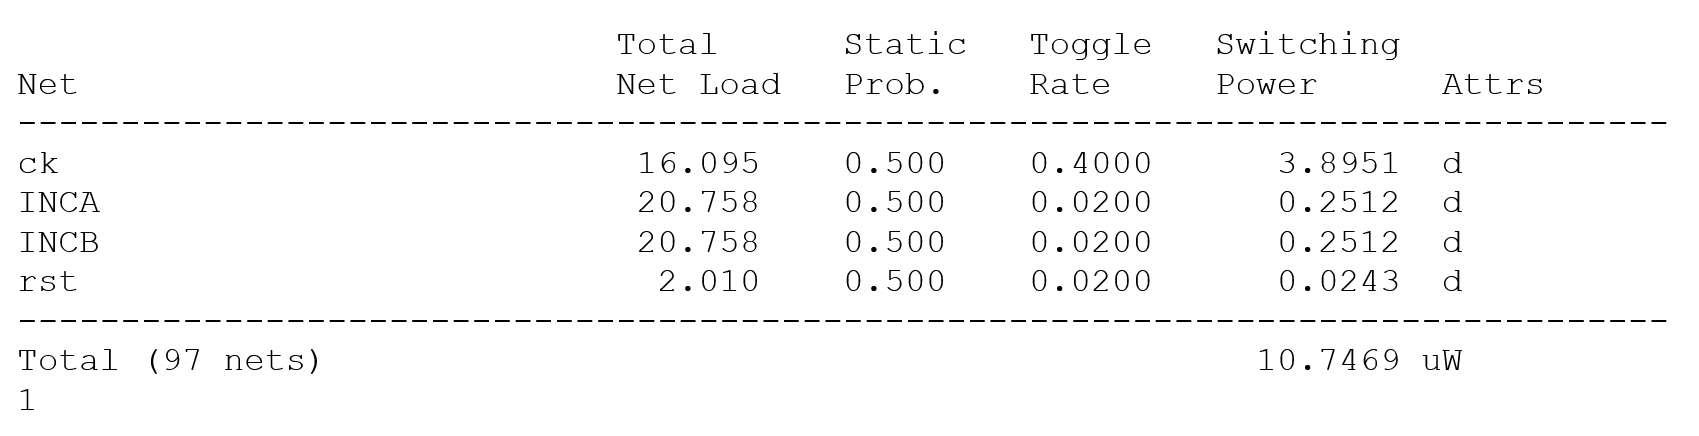
\includegraphics[scale=0.65]{immagini/3_8}
	\caption{\textit{Power report input nets}}
	\label{3_8}
\end{figure}
\newpage
Esattamente come prima è stata cambiata la probabilità di reset, clock e input per vedere come cambiano i valori di potenza, portandole rispettivamente a 0, 0.5, 0.12.
Si è eseguito il comando \textit{report\_power -include\_input\_nets} e si sono analizzati i report di potenza che sono riportati in Figura \ref{3_9} e \ref{3_10}.\\
\begin{figure}[!htb]
	\centering
	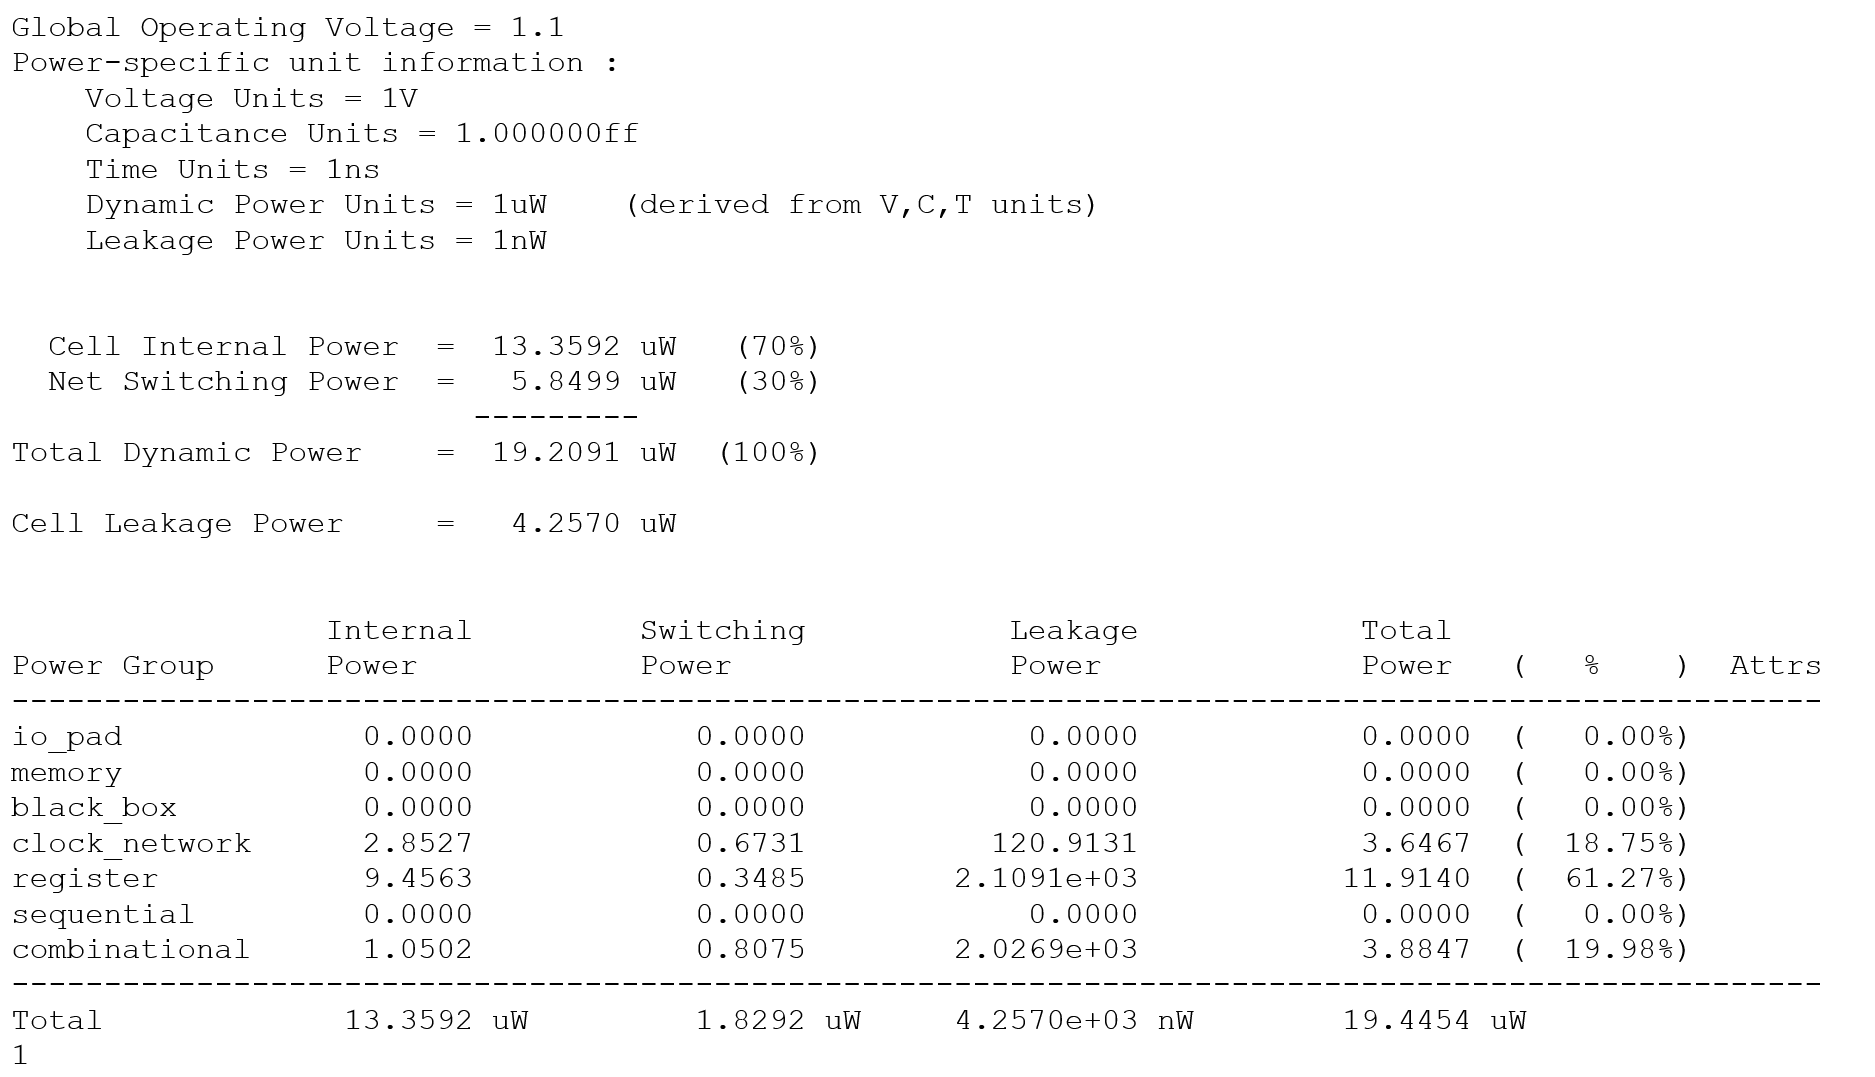
\includegraphics[scale=0.65]{immagini/3_9}
	\caption{\textit{Power report circuito con clock gating e probabilità ingressi modificate}}
	\label{3_9}
\end{figure}
\begin{figure}[!htb]
	\centering
	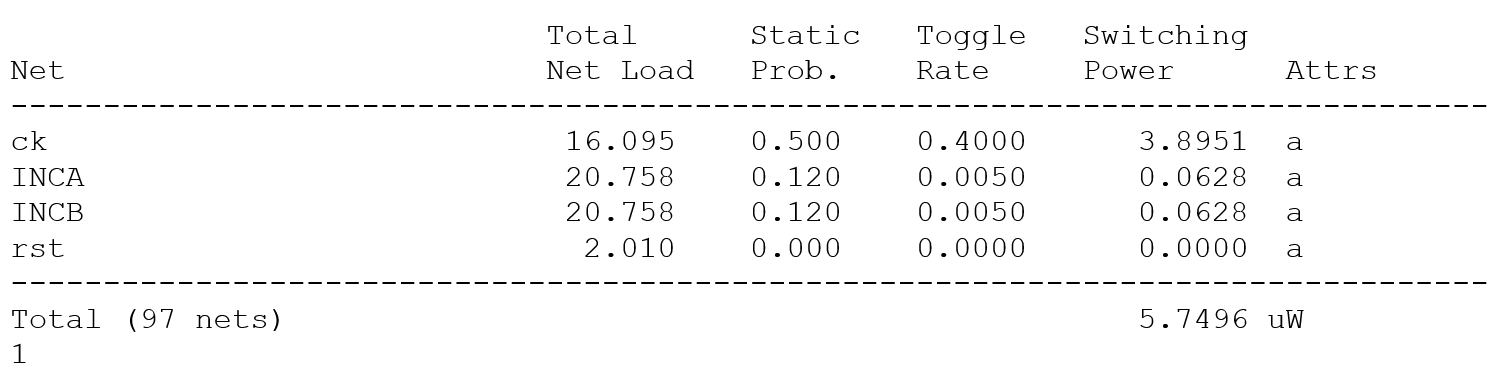
\includegraphics[scale=0.65]{immagini/3_10}
	\caption{\textit{Power report input nets}}
	\label{3_10}
\end{figure}
\newpage

Si può notare come si è ottenuto un risparmio del 41\% rispetto al caso senza Clock Gating. \\
Infine si ri-esegue l'analisi tramite il report cell, raffigurato in Figura \ref{3_11}. Si può notare come ora il numero di celle sia aumentato e con esso anche l'area.\\
Rispetto al caso senza Clock Gating si ha ora un'area pari a $238.0700005 \mu m^{2}$ e un numero di celle pari a 78. L'aumento dell'area è uno degli svantaggi della tecnica che Clock Gating, ma comunque, in questa situazione, si tratta di un incremento pari solo al 3.47\%, che risulta assolutamente accettabile visto che comporta un risparmio di potenza pari al 41\%.
\begin{figure}[!htb]
	\centering
	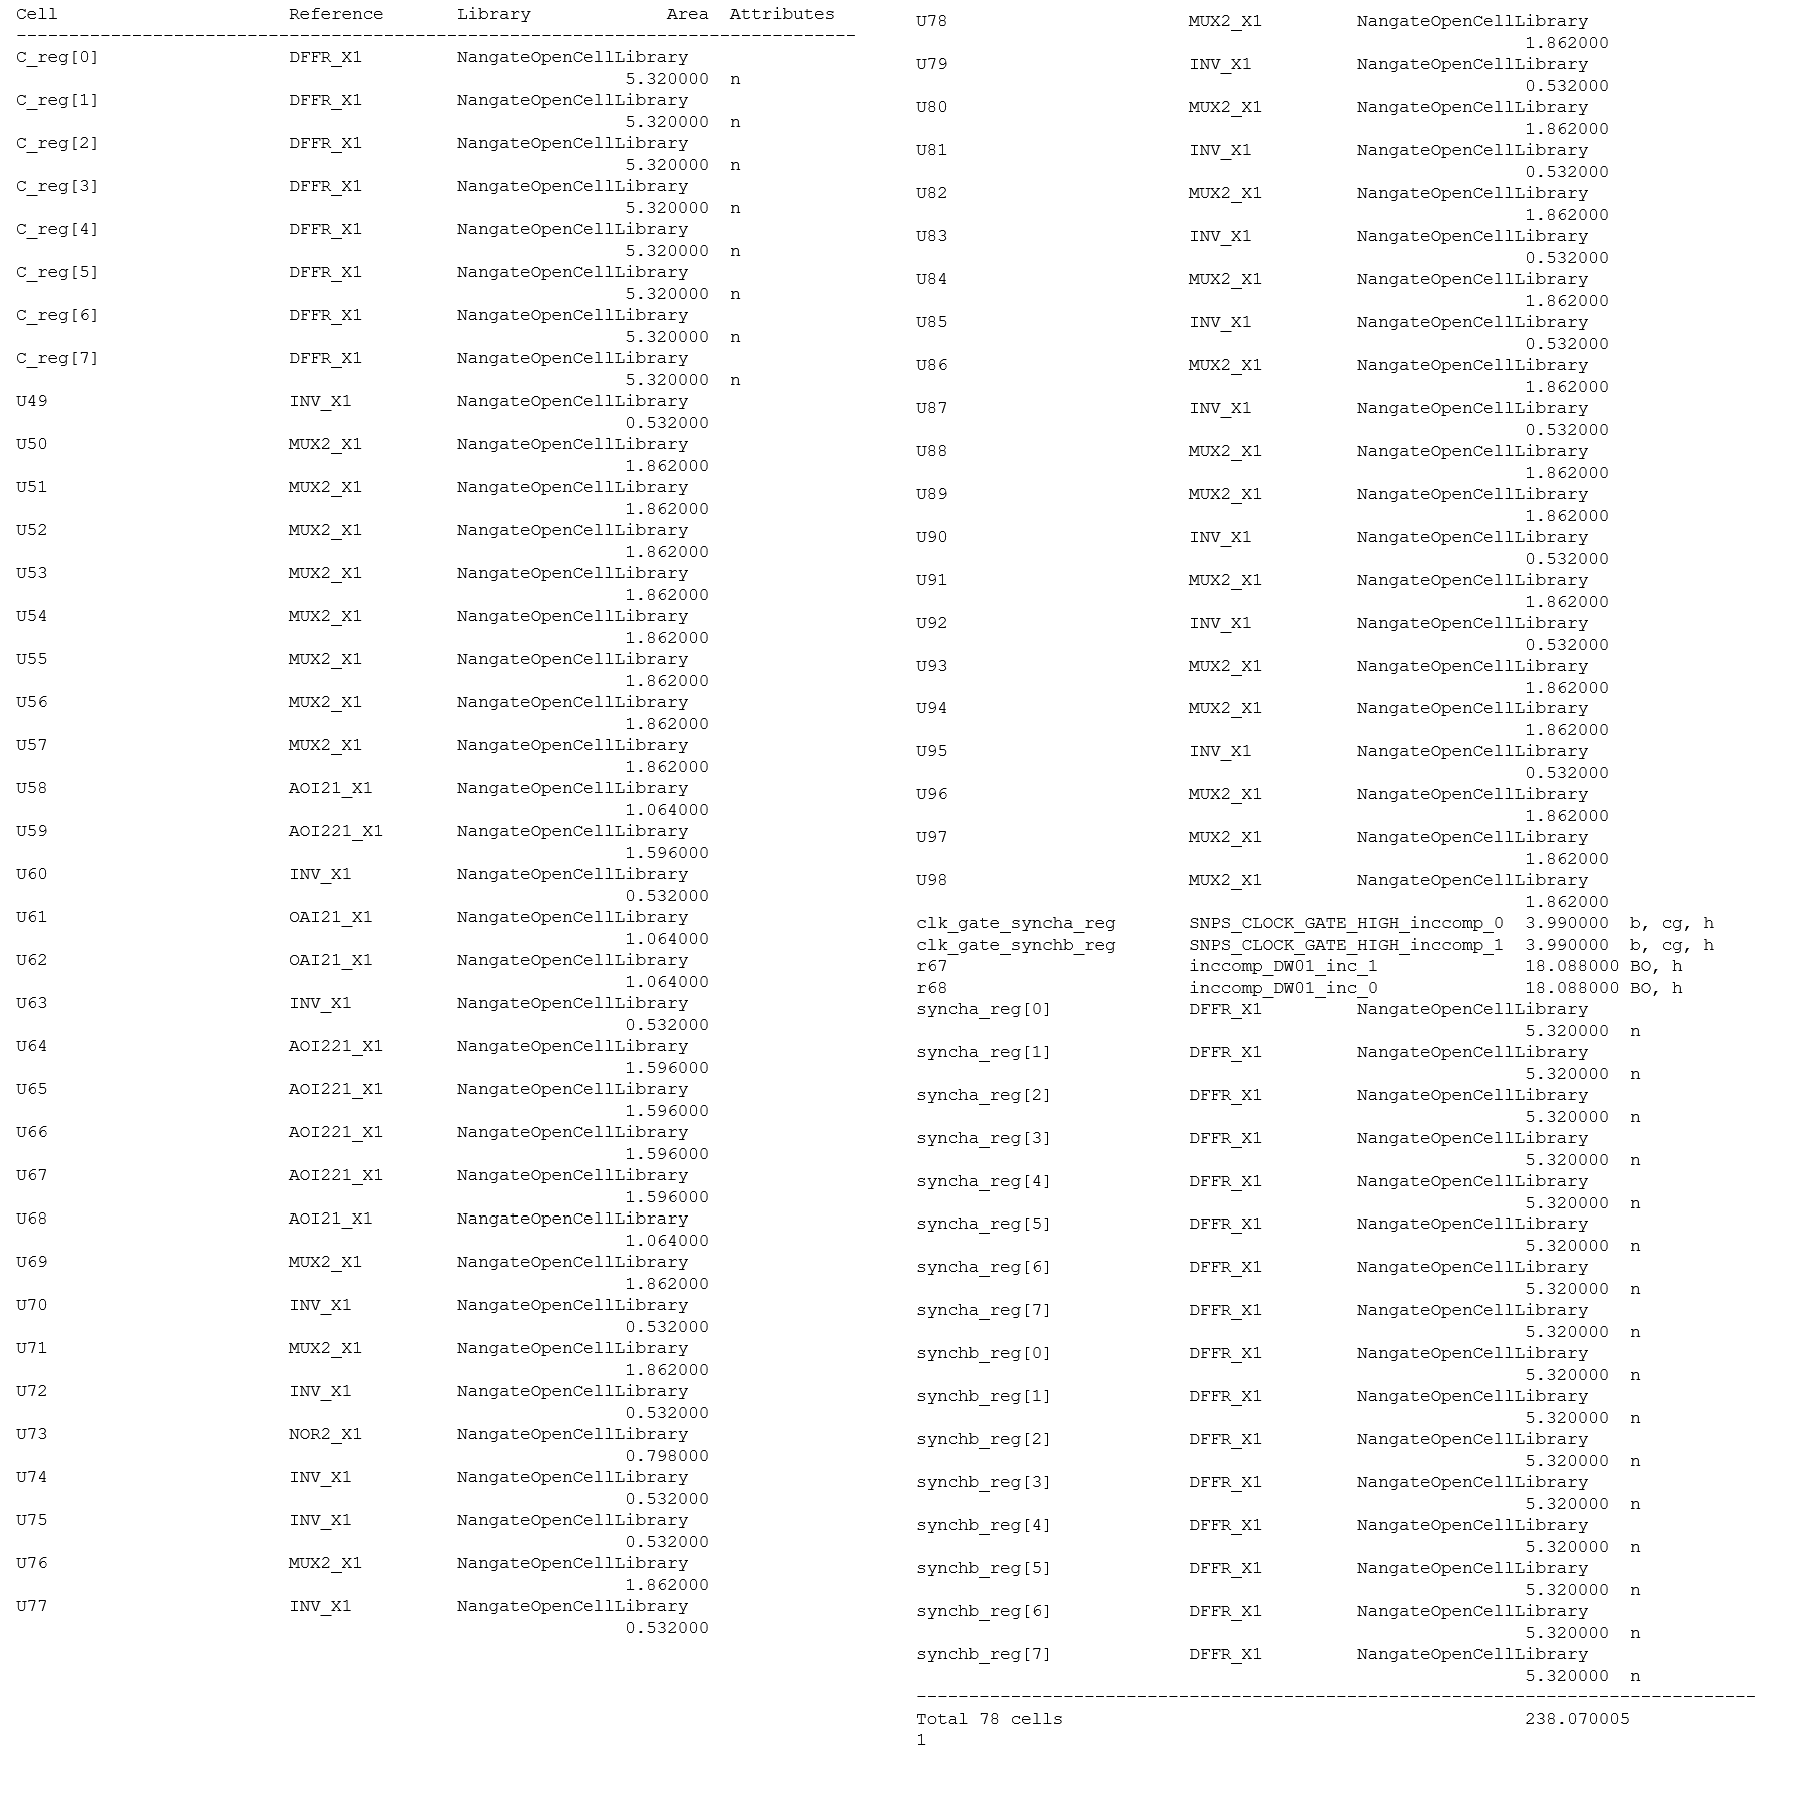
\includegraphics[scale=0.65]{immagini/3_11}
	\caption{\textit{Report cell con clock gating}}
	\label{3_11}
\end{figure}

\subsection{Some more clock gating?}
Il codice VHDL fornito è scritto in modo tale che il sintetizzatore non applichi la tecnica del Clock Gating sul registro di uscita: la motivazione risiede nell'utilizzo del costrutto \textit{if-else}, in quanto nel codice iniziale non venivano dichiarati tutti i possibili casi tramite \textit{elsif}. Modificando opportunamente il codice VHDL,  riportato per interezza in appendice Figura \ref{3_vhdl}, e inserendo le linee di codice riportate in Figura \ref{3_vhdl_2}, il sintetizzatore inserisce un blocco di clock gating sul registro di uscita perchè interpreta che potrebbero esserci condizioni in cui non si andrà a scrivere sul registro di uscita.
\begin{figure}[!htb]
	\centering
	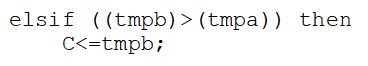
\includegraphics[scale=1.5]{immagini/3_vhdl_2}
	\caption{\textit{estratto modifiche al vhdl}}
	\label{3_vhdl_2}
\end{figure}

\noindent Le modifiche al VHDL hanno portato al risultato richiesto, come si può notare in Figura \ref{3_12} che riporta il circuito sintetizzato e in Figura \ref{3_13} che riporta il particolare del blocco di Clock Gating inserito dal sintetizzatore.
\\
\begin{figure}[!htb]
	\centering
	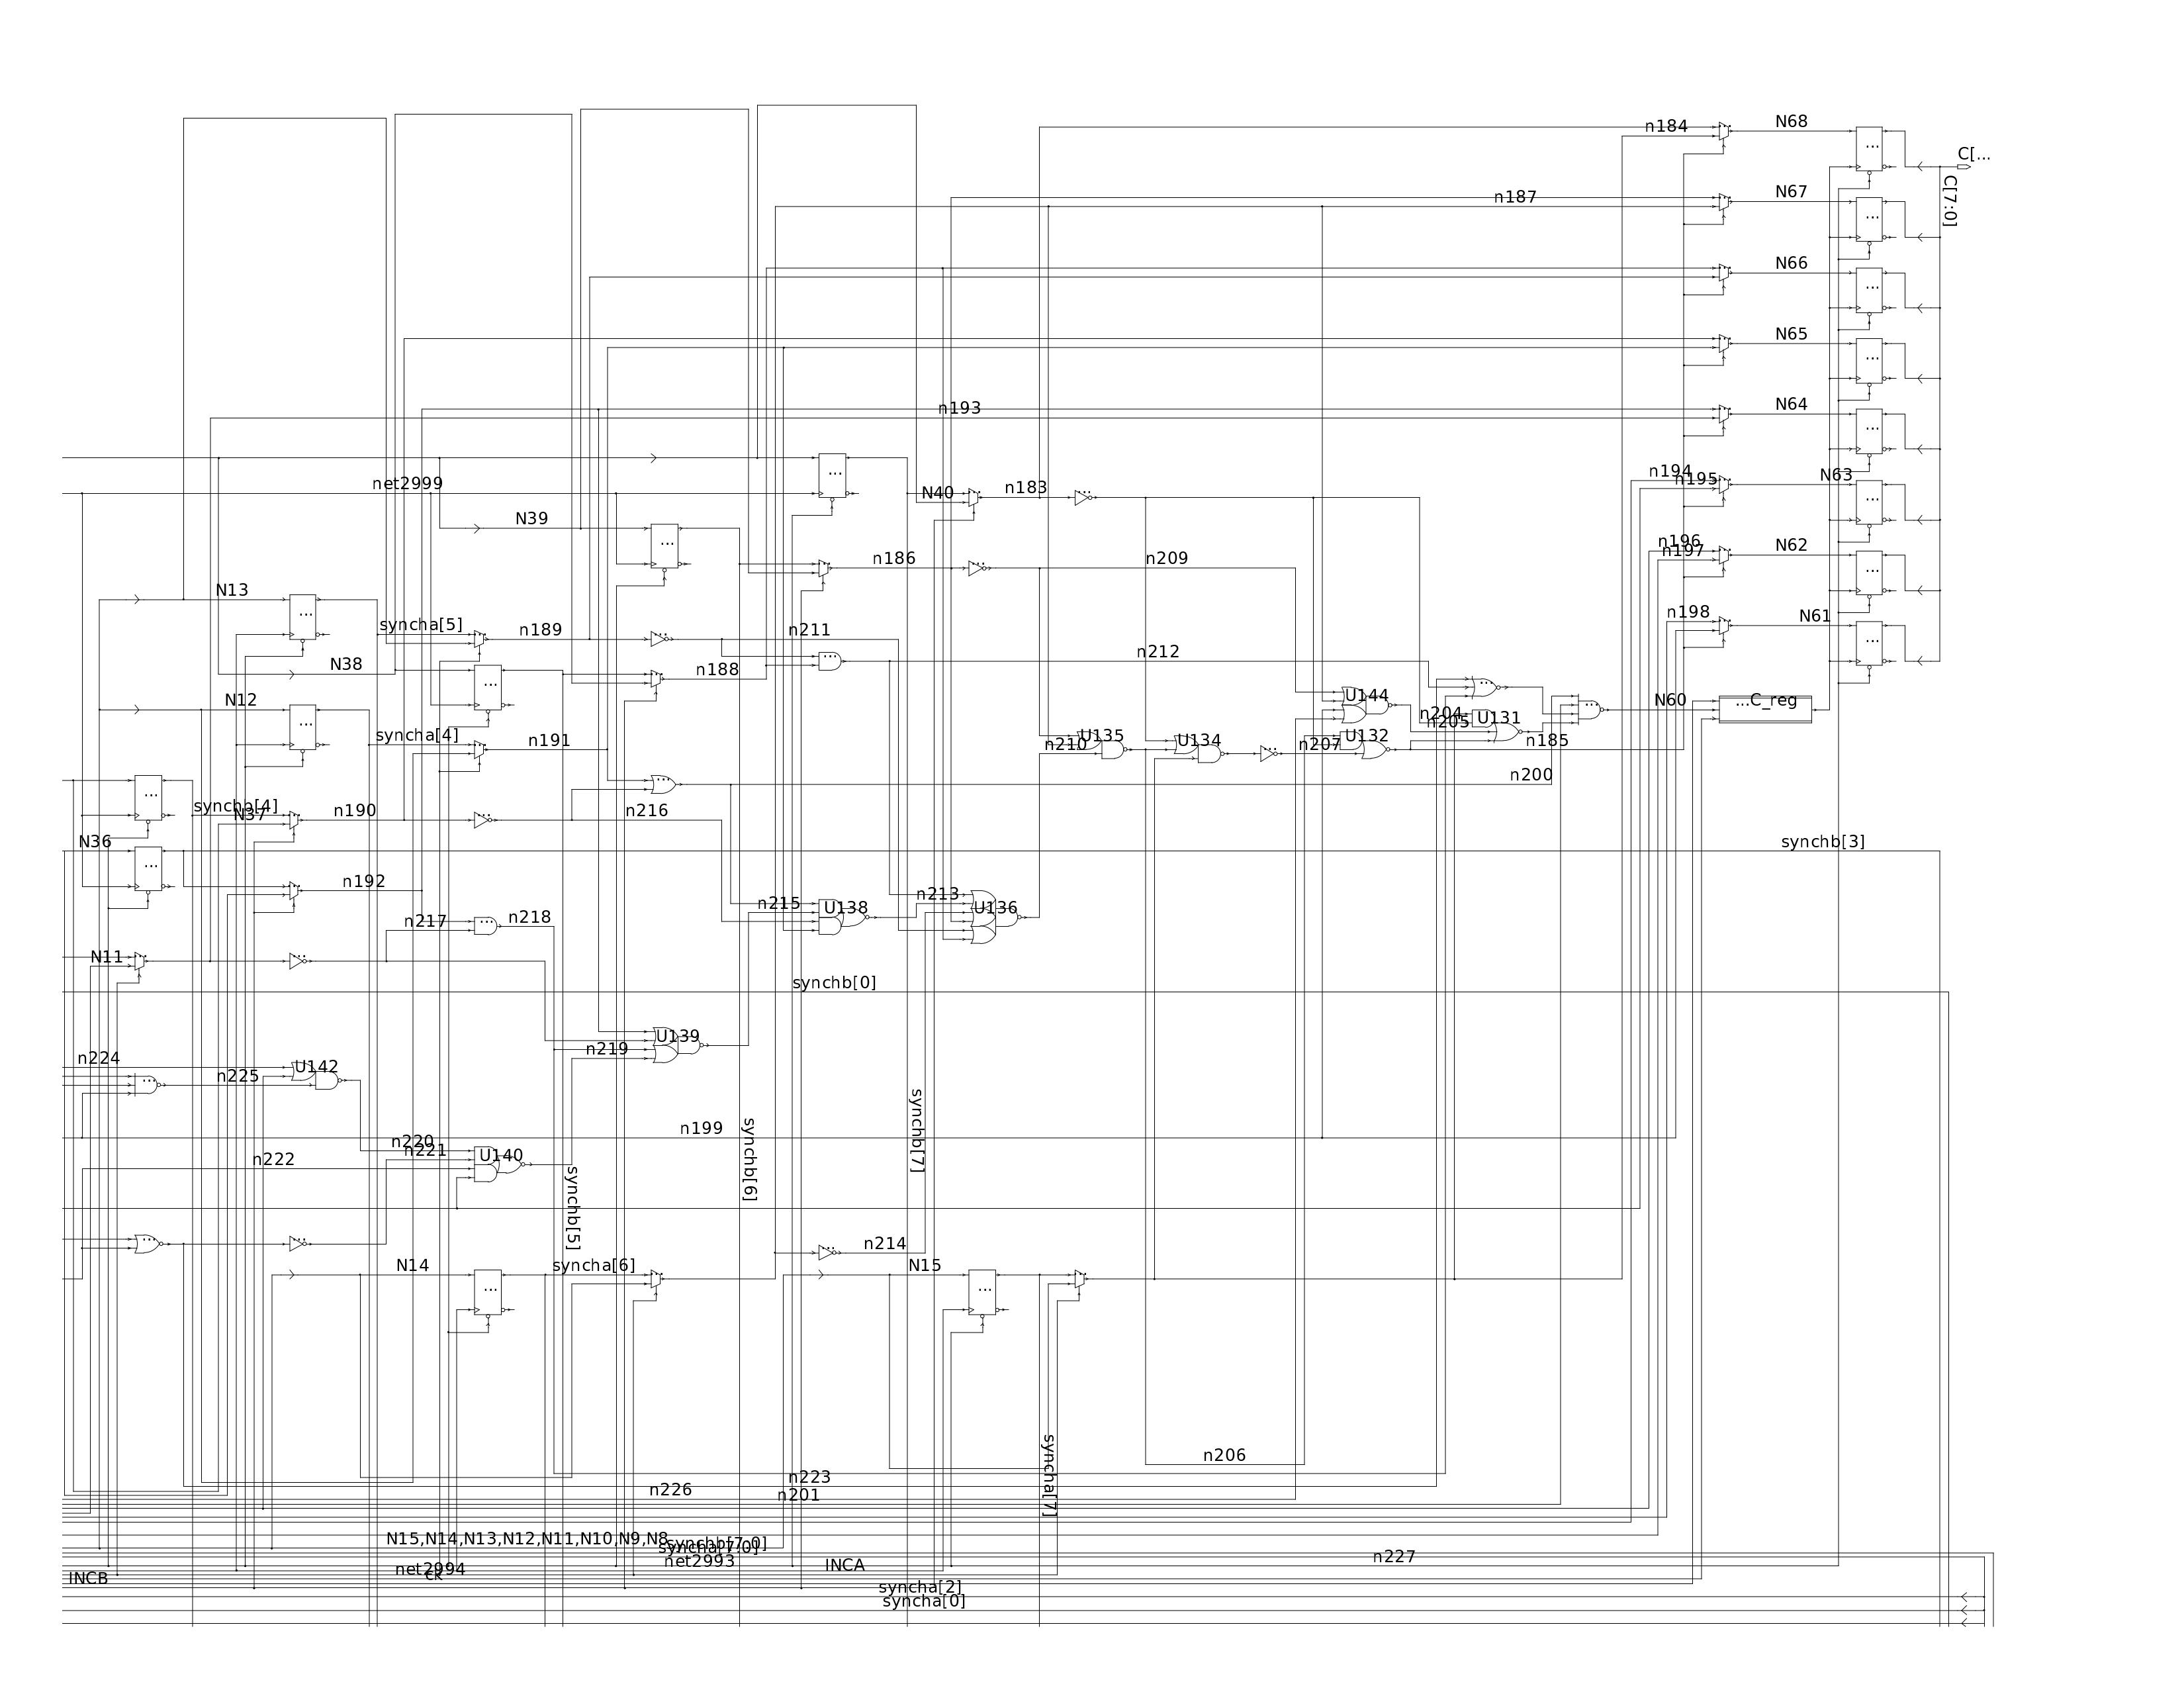
\includegraphics[scale=0.5]{immagini/3_12}
	\caption{\textit{circuito sintetizzato}}
	\label{3_12}
\end{figure}
\begin{figure}[!htb]
	\centering
	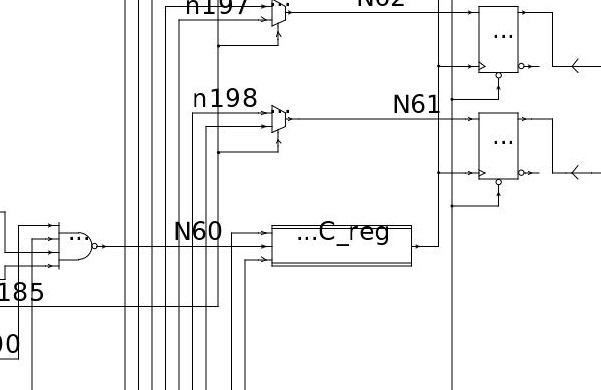
\includegraphics[scale=1.5]{immagini/3_13}
	\caption{\textit{particolare del blocco di clock gating sull'uscita}}
	\label{3_13}
\end{figure}
\\
Si eseguono ora le analisi dei consumi, esattamente come nel punto precedente.\\
Le prima analisi viene svolta senza la tecnica del Clock Gating e vengono lasciati i valori di Toggle Rate di default, quindi a 0.5. I power report ricavati sono riportati in Figura \ref{elsif1} e \ref{elsif2}.
\begin{figure}[!htb]
	\centering
	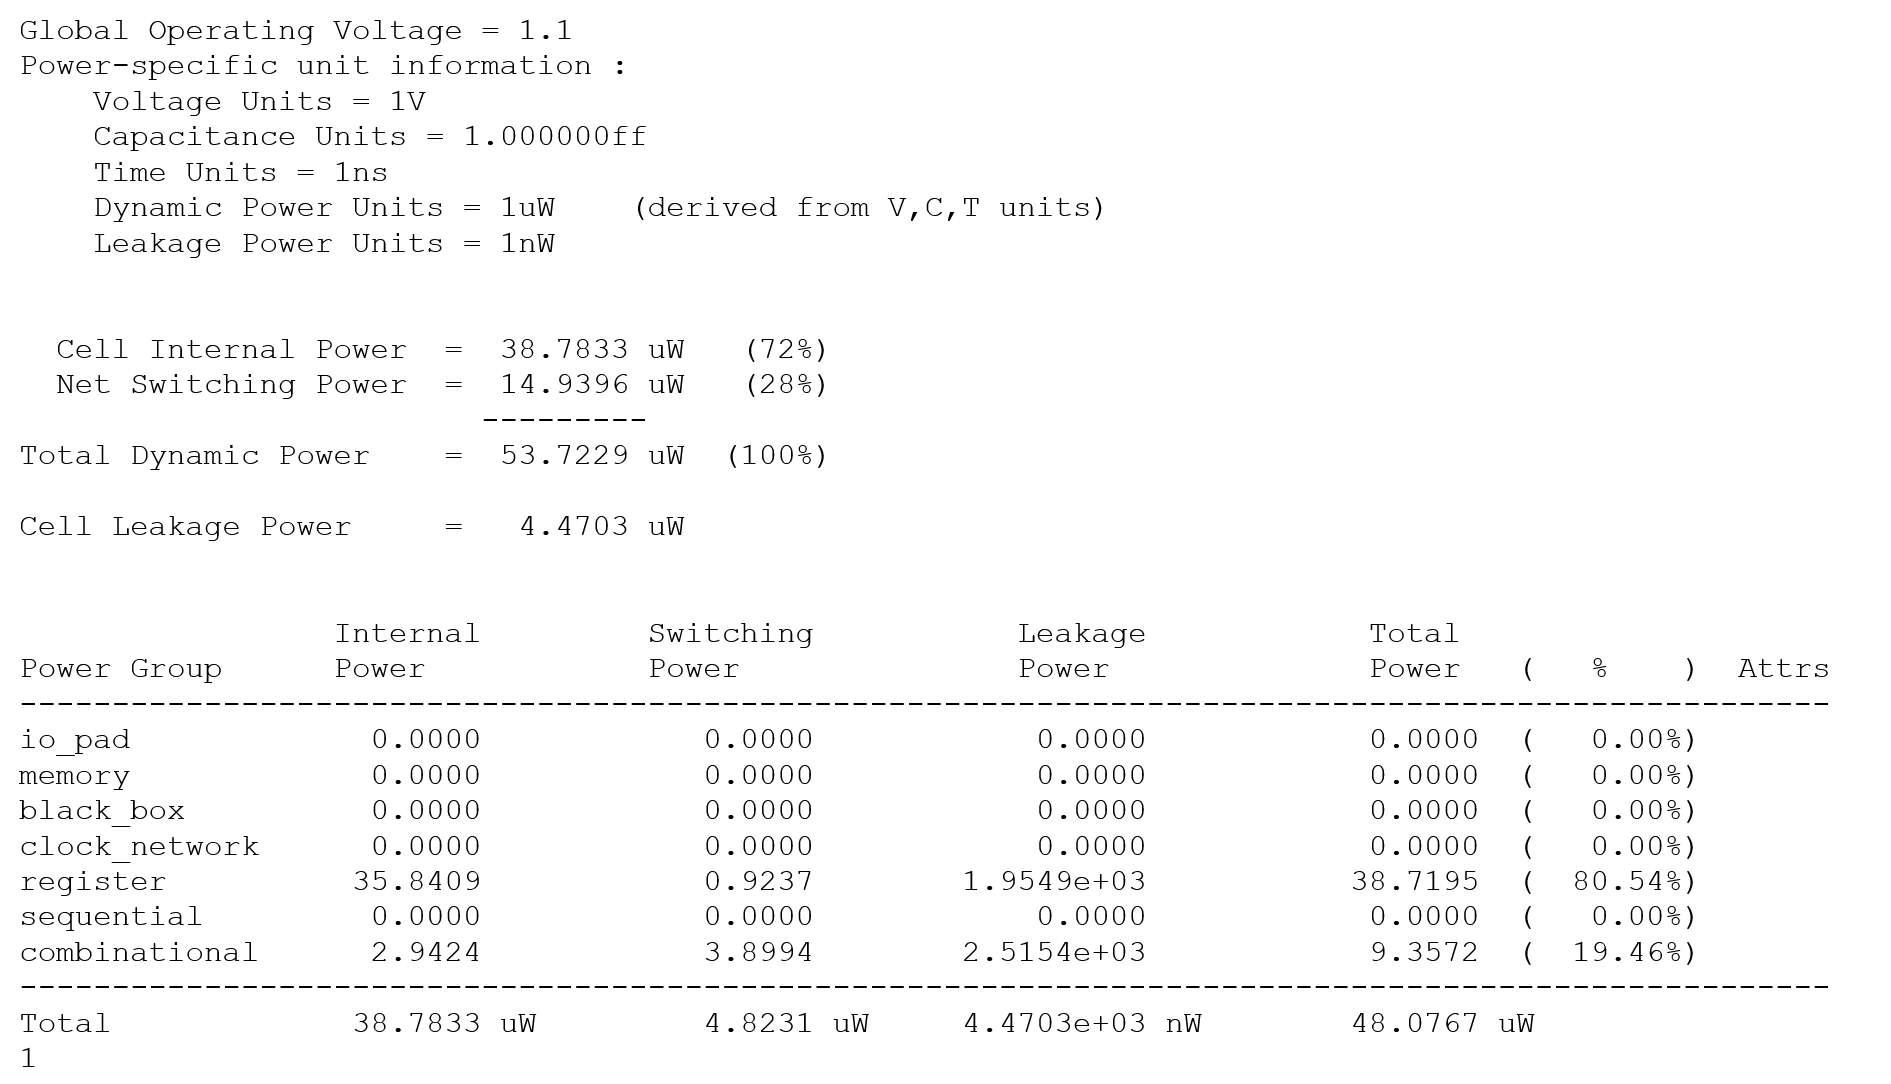
\includegraphics[scale=0.65]{immagini/elsif1}
	\caption{\textit{Power report senza clock gating con toggle rate pari a 0.5}}
	\label{elsif1}
\end{figure}
\begin{figure}[!htb]
	\centering
	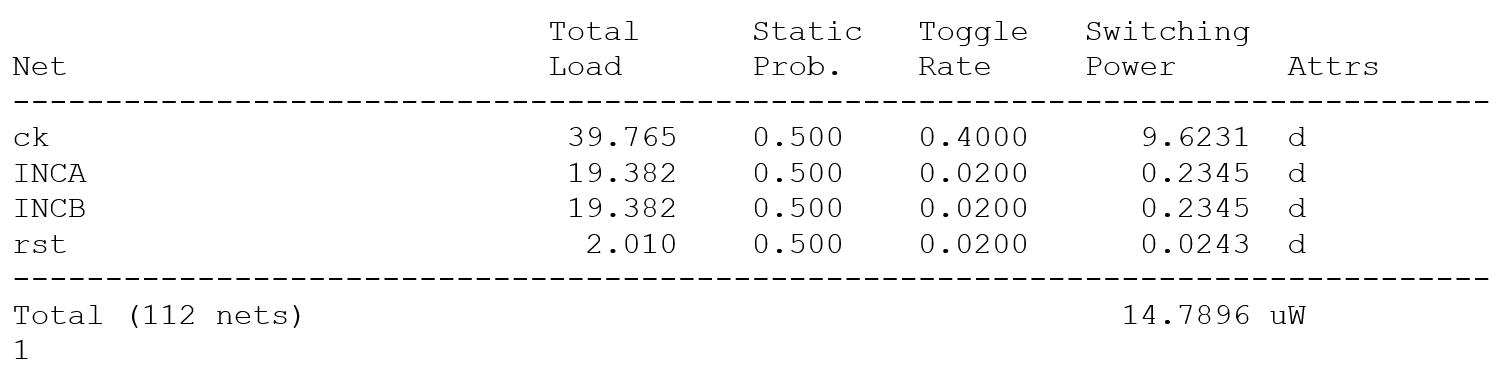
\includegraphics[scale=0.65]{immagini/elsif2}
	\caption{\textit{Power report input nets senza clock gating}}
	\label{elsif2}
\end{figure}
\\
Si può ben notare come rispetto al caso precedente, la potenza sia leggermente aumentata in quanto, avendo aggiunto un blocco di Clock Gating prima del registro di uscita, sono aumentati i gate totali che quindi portano ad una maggiore dissipazione di potenza. \\
Viene ora modificato il Toggle Rate del clock, del reset e degli ingressi, ottenendo i report in Figura \ref{elsif3} e \ref{elsif4}. Come ci si aspettava l'aggiunta del blocco in uscita ha portato a una diminuzione della potenza. \\
\begin{figure}[!htb]
	\centering
	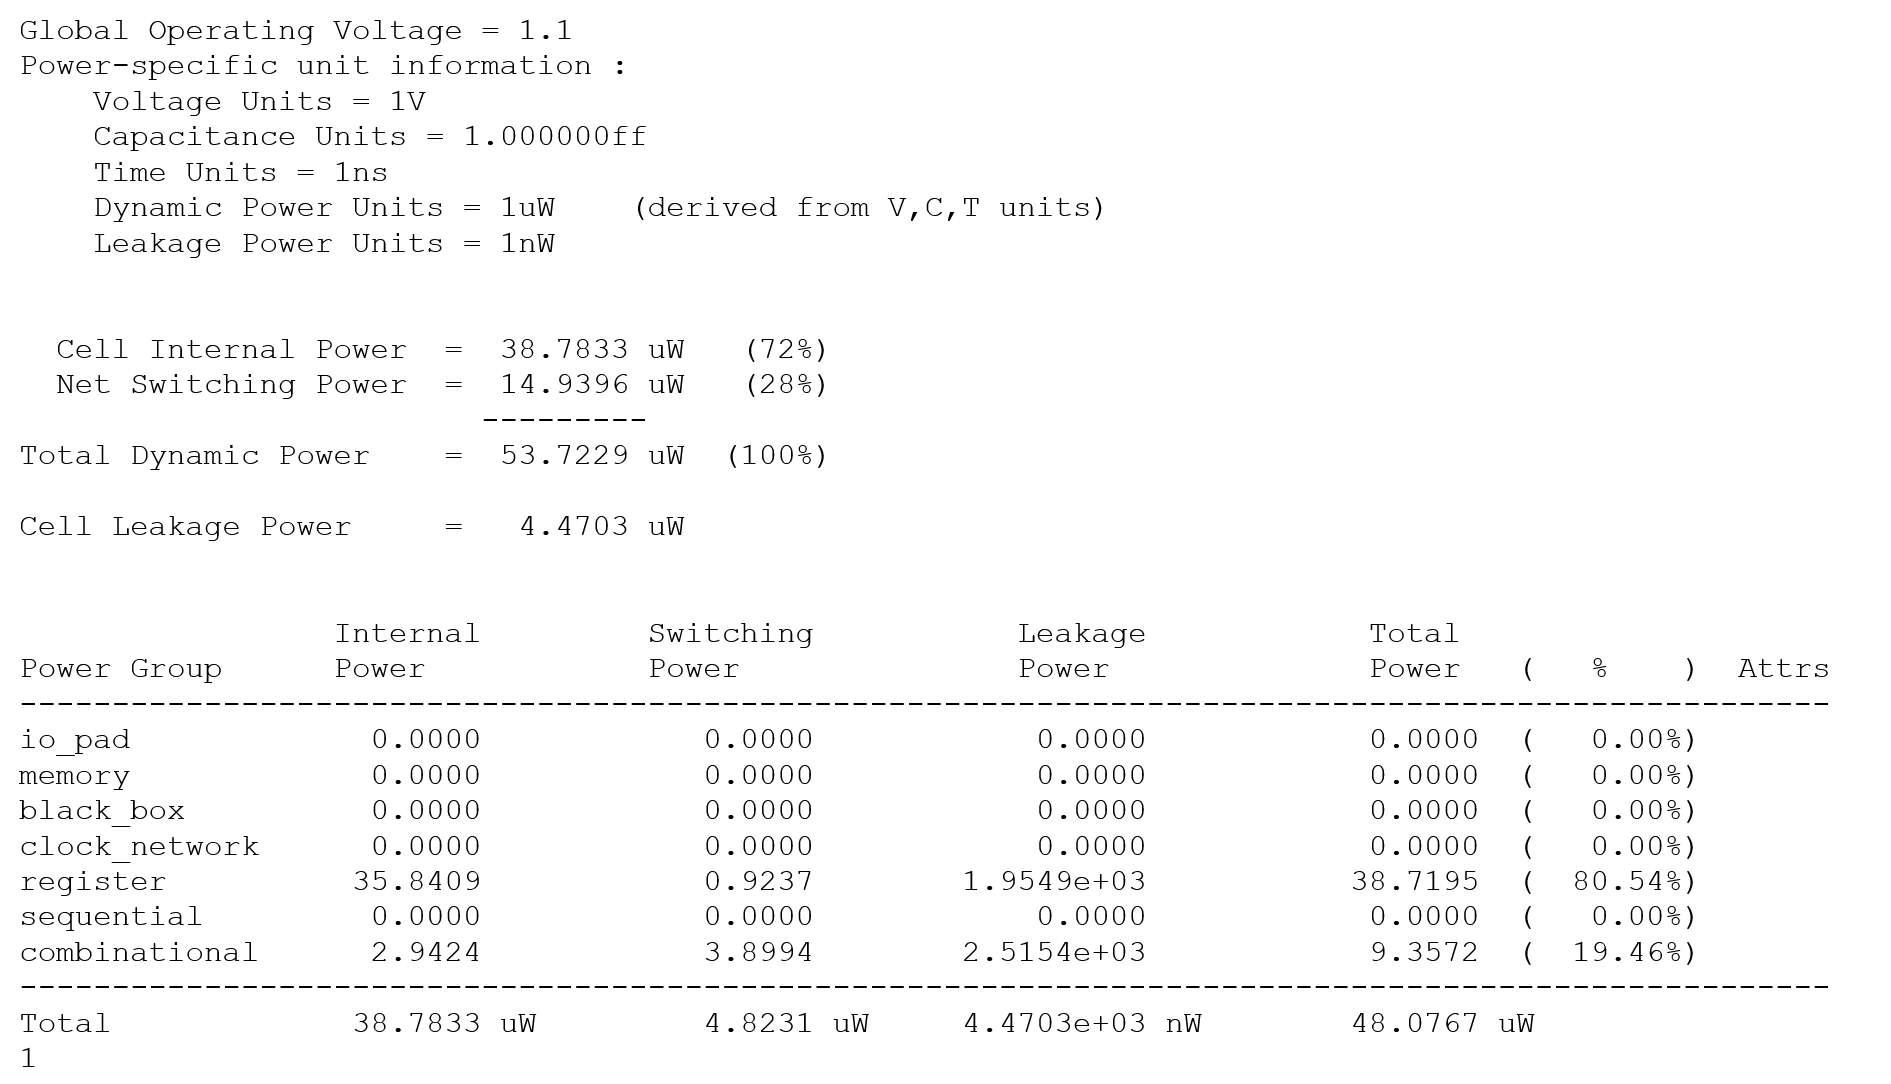
\includegraphics[scale=0.65]{immagini/elsif1}
	\caption{\textit{Power report circuito senza clock gating con toggle rates modificati}}
	\label{elsif3}
\end{figure}
\begin{figure}[!htb]
	\centering
	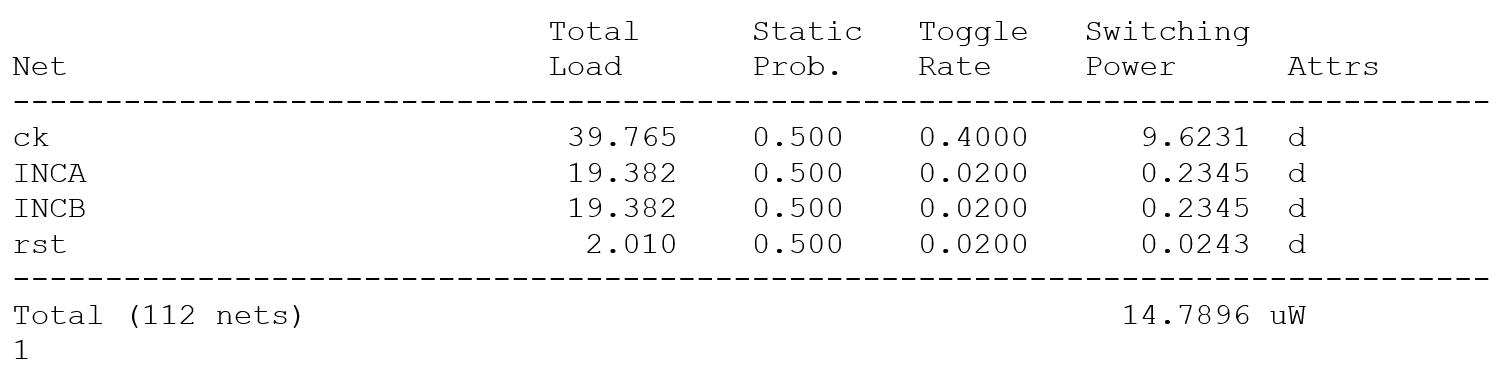
\includegraphics[scale=0.65]{immagini/elsif2}
	\caption{\textit{Power report input nets senza clock gating}}
	\label{elsif4}
\end{figure}
\\
Si esegue infine il comando \textit{report cell} per ottenere l'area e il numero di celle utilizzate per la sintesi. Il report viene raffigurato i Figura \ref{elsif5}. \\
\newpage
\begin{figure}[!htb]
	\centering
	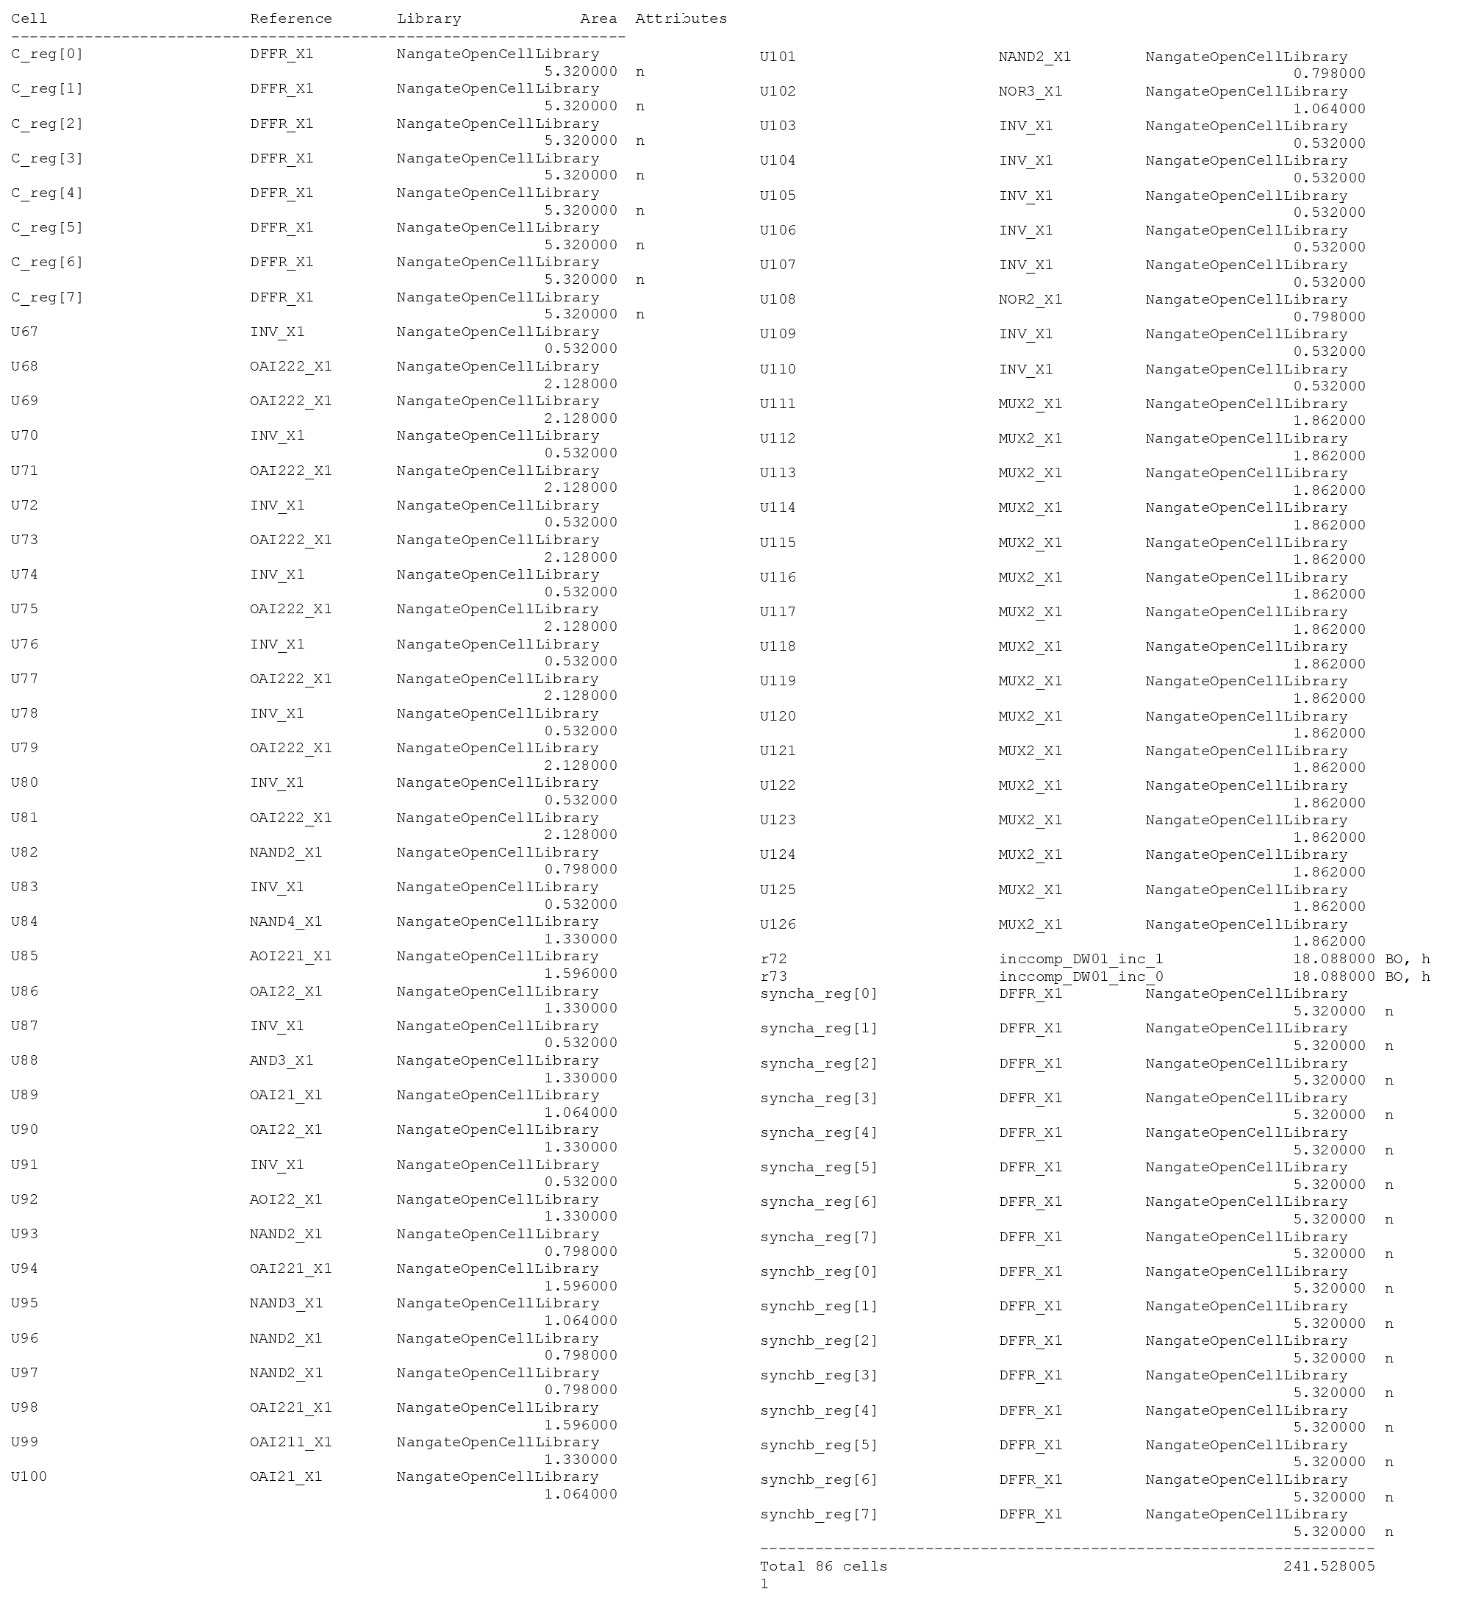
\includegraphics[scale=0.25]{immagini/elsif5}
	\caption{\textit{Power cell senza clock gating}}
	\label{elsif5}
\end{figure}
\noindent Si può ben notare che ora il numero di celle è leggermente aumentato e di conseguenza anche l'area, in quanto si è aggiunta una logica prima del registro di uscita.\\
Si analizza allo stesso modo il circuito con l'aggiunta della tecnica del Clock Gating. Tutti i report, con lo stesso ordine dei punti precedenti, vengono riportati nelle Figure \ref{elsif6}, \ref{elsif7}, \ref{elsif8},\ref{elsif9}.\\
\begin{figure}[!htb]
	\centering
	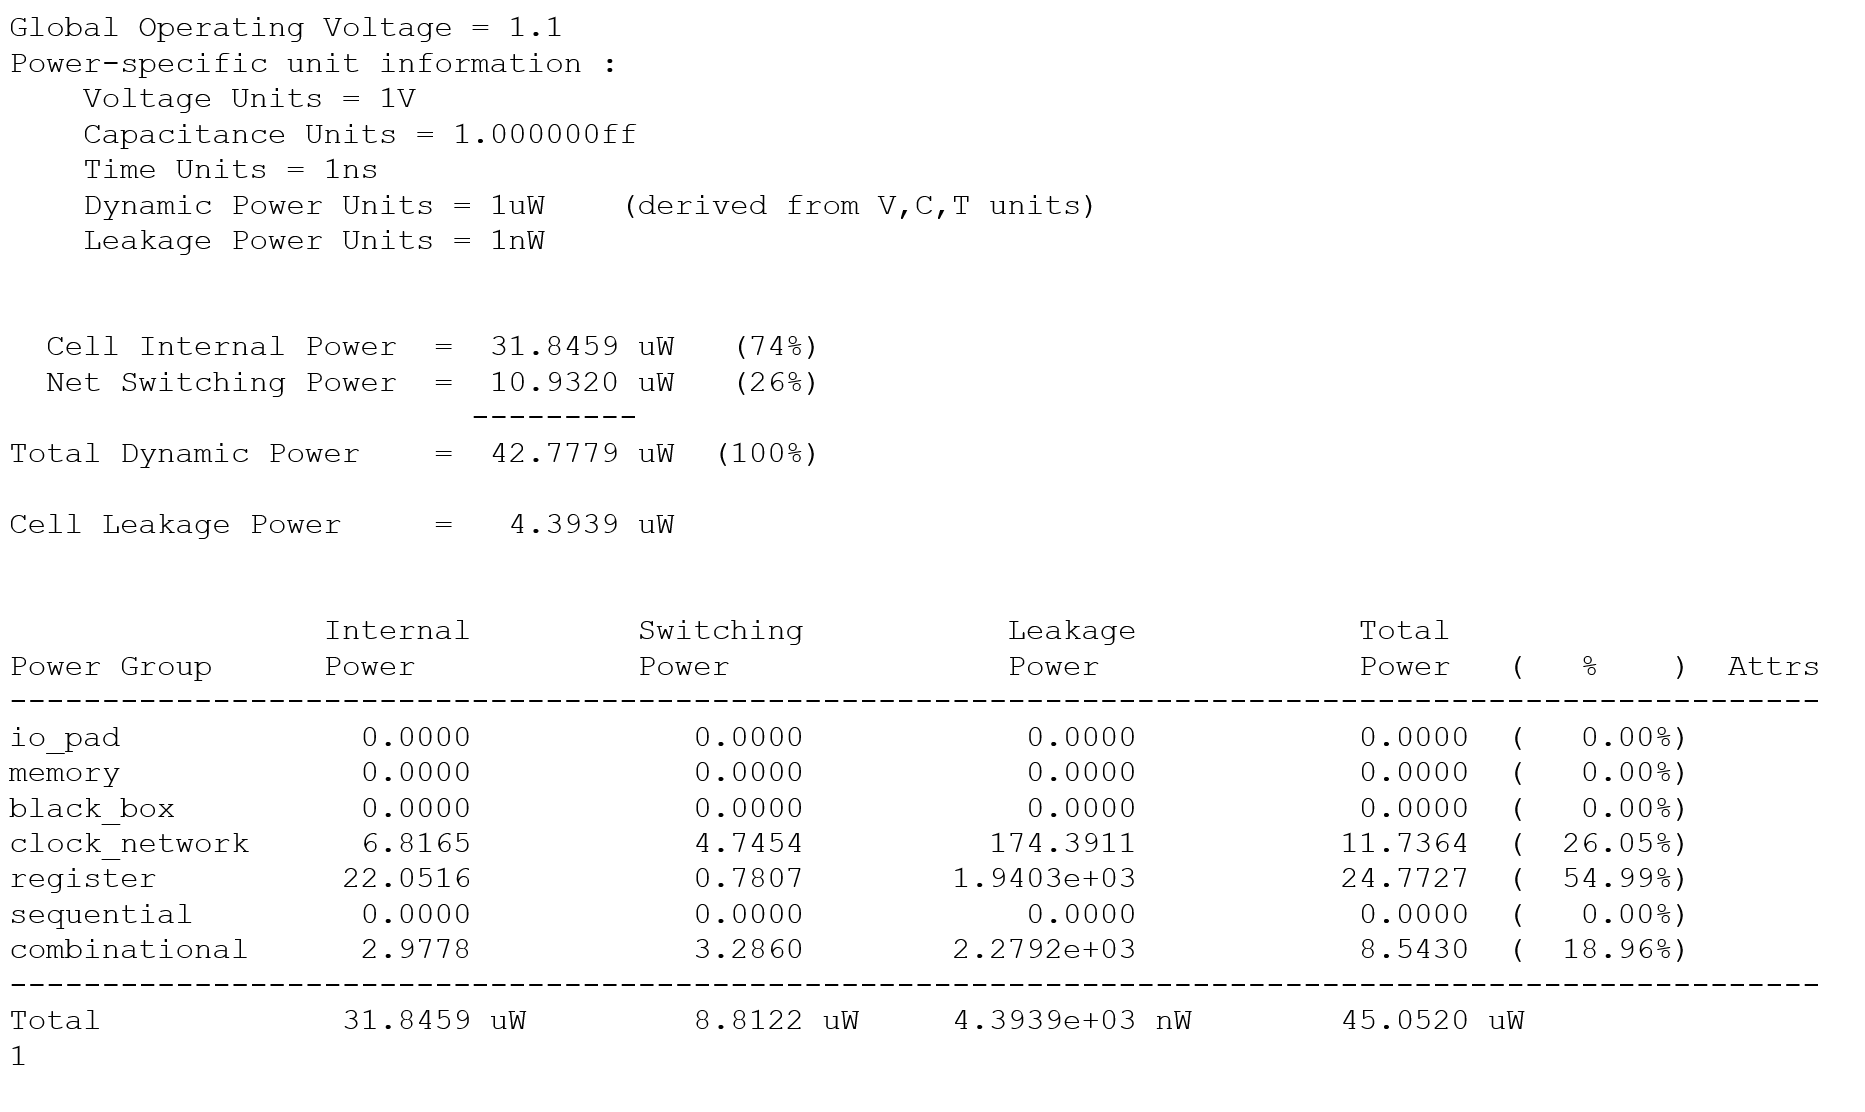
\includegraphics[scale=0.65]{immagini/elsif6}
	\caption{\textit{Power report circuito con clock gating e condizioni iniziali}}
	\label{elsif6}
\end{figure}
\begin{figure}[!htb]
	\centering
	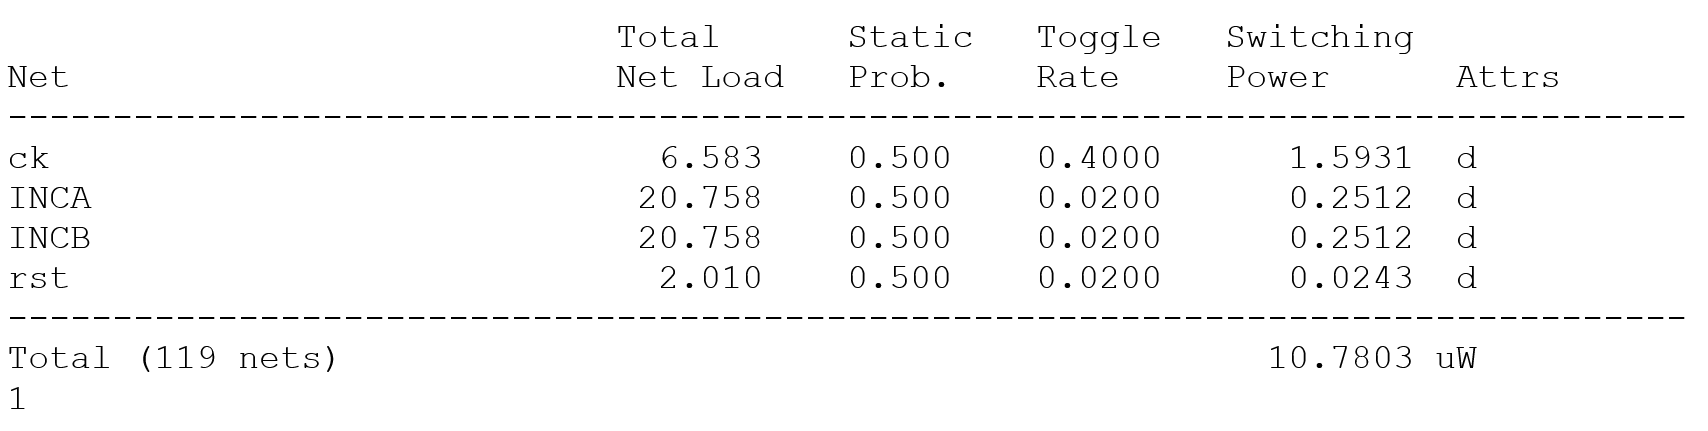
\includegraphics[scale=0.65]{immagini/elsif7}
	\caption{\textit{Schema implementativo della tecnica del Clock Gating}}
	\label{elsif7}
\end{figure}
\begin{figure}[!htb]
	\centering
	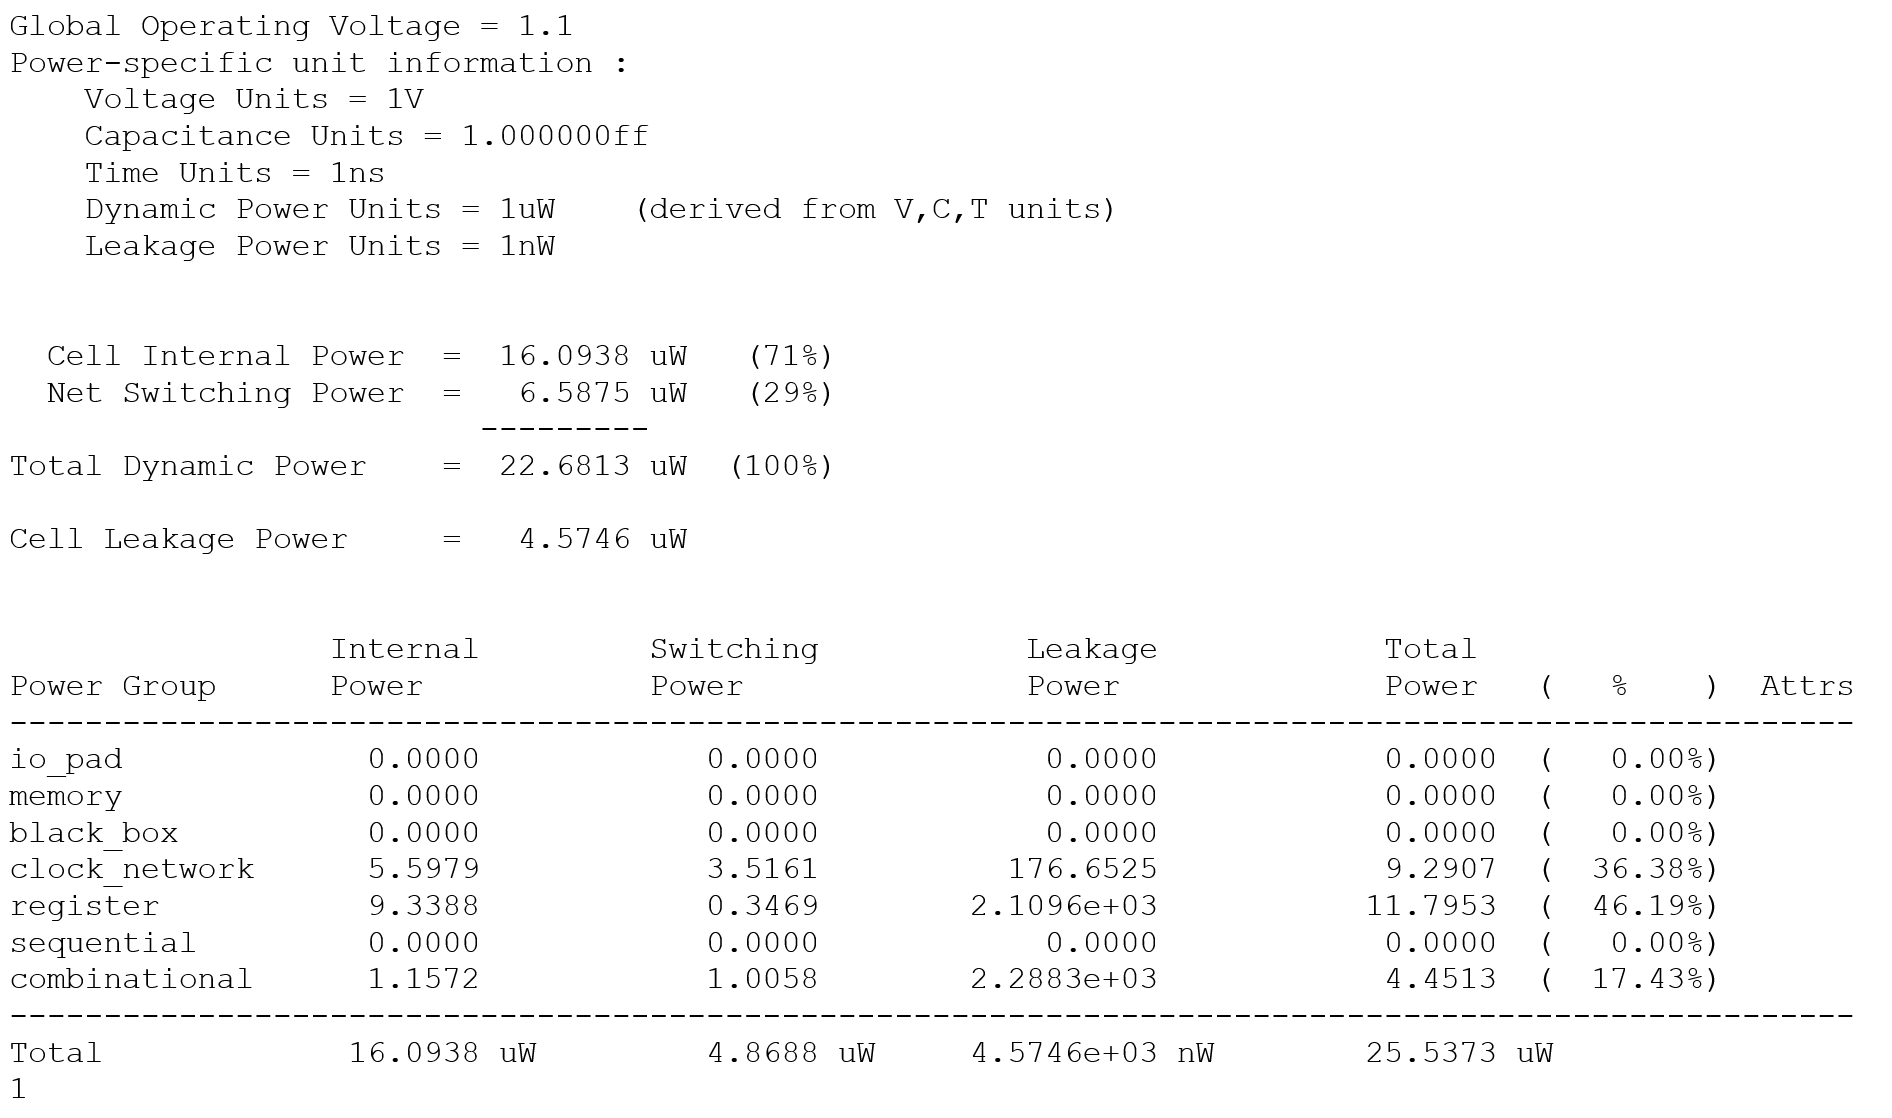
\includegraphics[scale=0.65]{immagini/elsif8}
	\caption{\textit{Schema implementativo della tecnica del Clock Gating}}
	\label{elsif8}
\end{figure}
\begin{figure}[!htb]
	\centering
	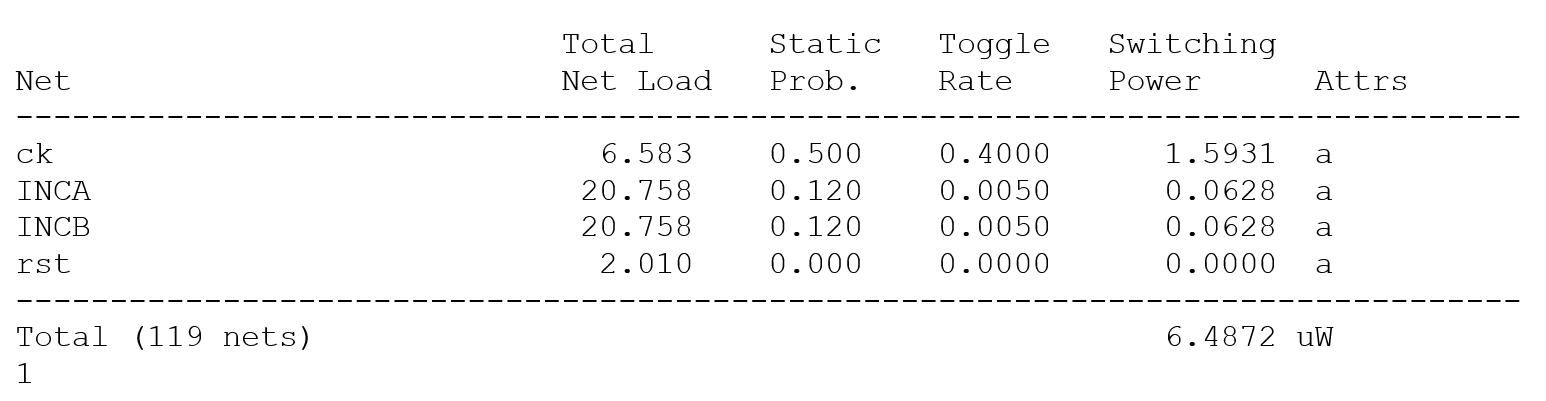
\includegraphics[scale=0.65]{immagini/elsif9}
	\caption{\textit{Schema implementativo della tecnica del Clock Gating}}
	\label{elsif9}
\end{figure}
\newpage
\noindent Si può ben notare come nell'ultimo caso, quindi con i Toogle Rate modificati rispetto ai valori di default, la potenza sia aumentata del 18\% rispetto al medesimo caso ma senza il blocco di Clock Gating prima del registro di uscita. Ovviamente se invece si confronta l'ultimo risultato con il risultato dell'analisi senza il Clock Gating, ma con il blocco in uscita, si ottiene un risparmio di potenza considerevole.\\
Come ultima analisi si esegue il \textit{report cell} di quest'ultimo caso, riportato in Figura \ref{elsif10}, che testimonia come l'applicazione di questa tecnica comporti un aumento dell'area occupata a causa dell'inserimeto di una logica di controllo.
\begin{figure}[!htb]
	\centering
	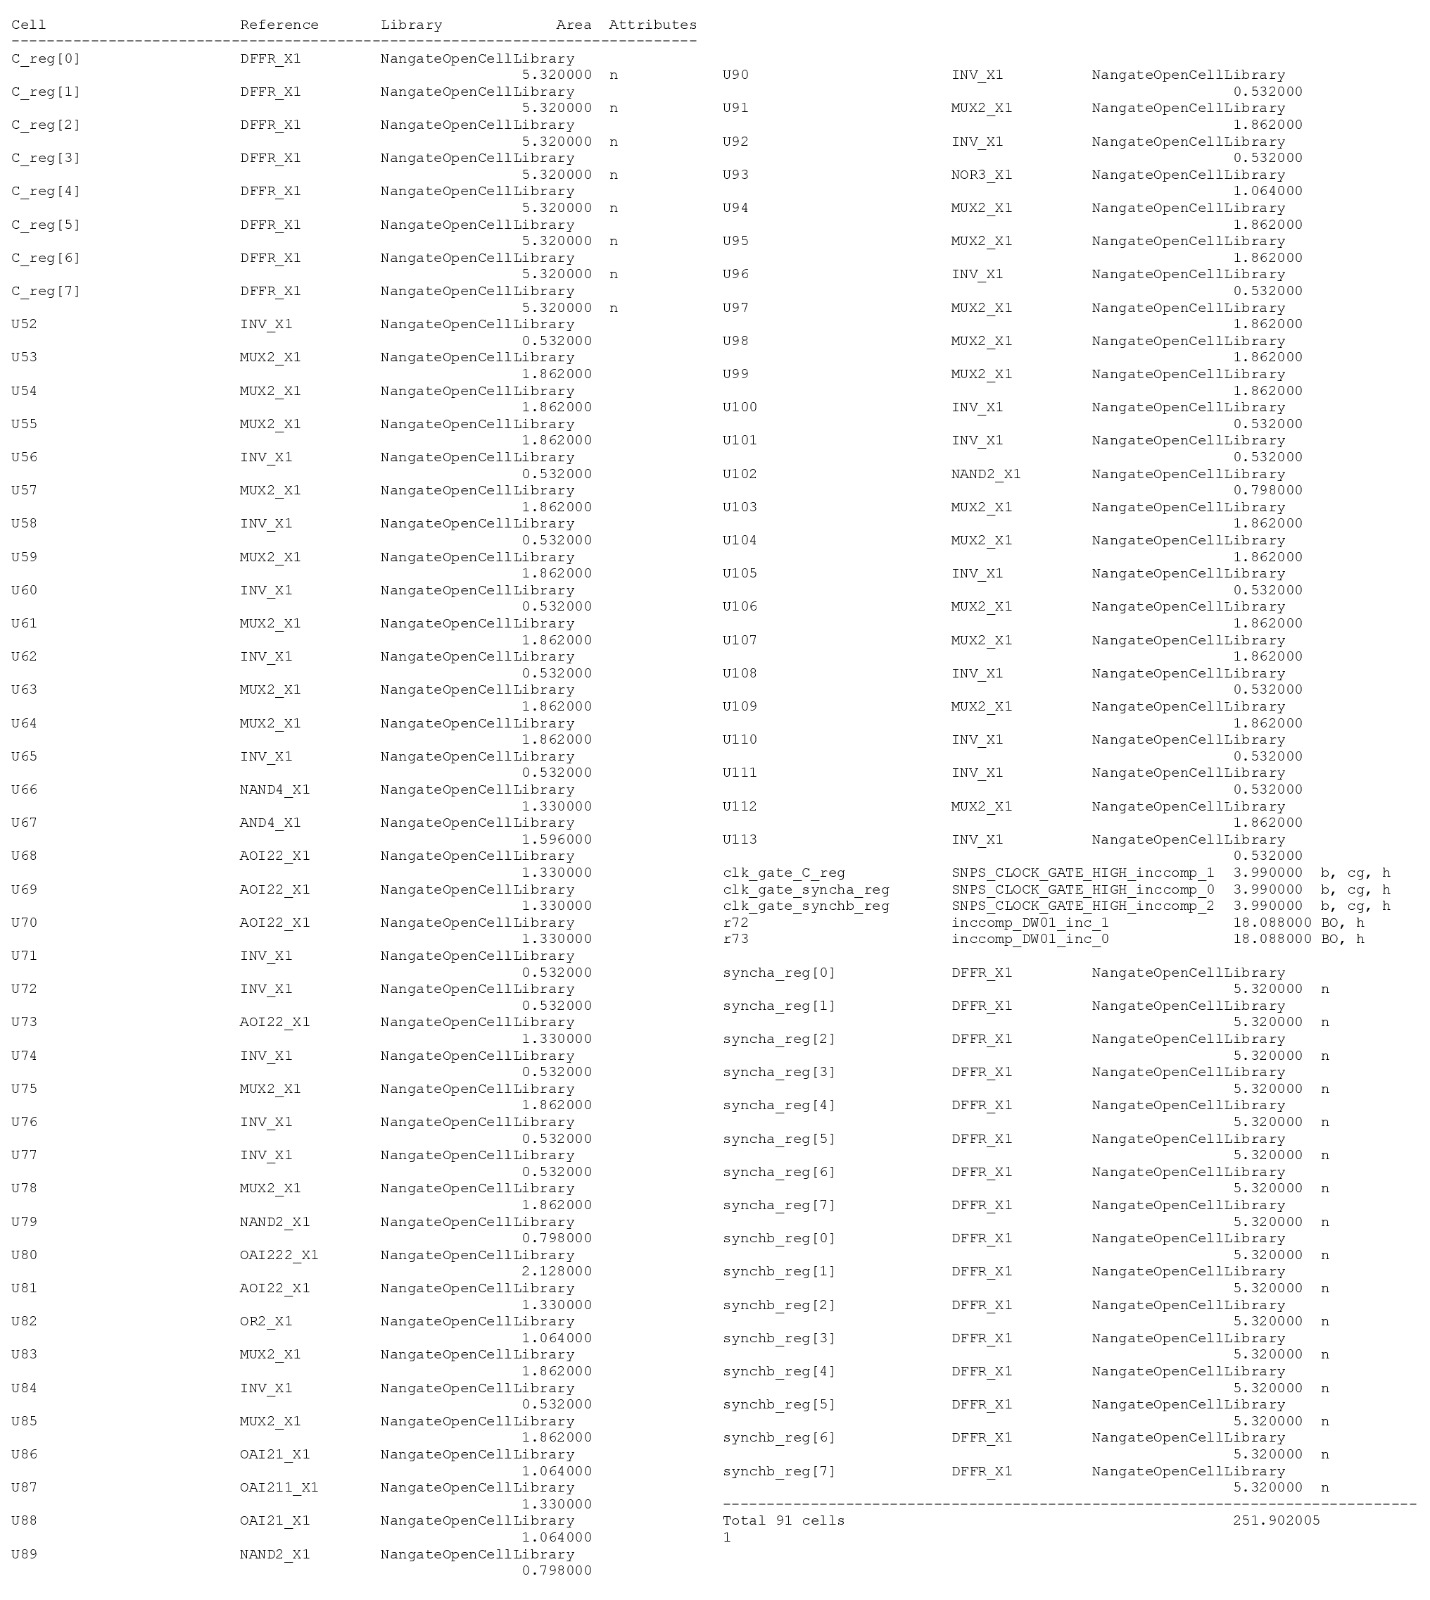
\includegraphics[scale=0.28]{immagini/elsif10}
	\caption{\textit{Schema implementativo della tecnica del Clock Gating}}
	\label{elsif10}
\end{figure}
\\
Per sintetizzare si confronta la potenza dinamica totale prima e dopo l'introduzione del Clock Gating nel registro di uscita e si riportano i valori nella Tabella \ref{Tab3_1}. Si può ben notare come la potenza nel secondo caso sia leggermente aumentata in quanto si introduce una logica di controllo più complessa che impatta sulla switching activity della macchina.
\begin{table}[!h]\footnotesize
	\centering
	\begin{tabular}{|c|c|}
		\hline
		& \textbf{Potenza Dinamica Totale}\\
		\hline
		Prima & $19.2091 \mu W$\\
		Dopo & $22.6813 \mu W$\\
		\hline
	\end{tabular}
	\caption{\textit{Risultati tempi NAND simulazione ELDO}}
	\label{Tab3_1}
\end{table}

\subsection{An automatic way to annotate activities}

\section{Pipelining and parallelizing}
Nella terza sezione dell'esercitazione si vede come si riesce a ridurre la potenza utilizzando la parallelizzazione e/o il pipelining. Si considera nuovamente il datapath del punto precedente, in Figura \ref{circuito_3_2}, di cui le caratteristiche di ritardo, potenza e occupazione di area sono riportate nella Tabella \ref{Tab33_1} nel caso in cui $V_{DD}=1 V$ e $f_{CLK}=5 MHz$.
\begin{table}[!h]\footnotesize
	\centering
	\begin{tabular}{|c|c|c|c|}
		\hline
		\textbf{Cell Type}& \textbf{Delay (ns)} & \textbf{Power ($\mu W @1 V, 5 MHz$)} & \textbf{Area ($\mu m^{2}$)} \\
		\hline
		\textit{REGISTER}& 2.0 (CK->Q) & 0.6 & 319 \\
	\textit{INCREMENT}& 40.0 & 2.55 & 256.0 \\
		\textit{COMPARATOR} & 84.0 & 2.16 & 161.0\\
		\textit{MUX} & 14.0 & 1.67& 117.0\\
		\hline
	\end{tabular}
	\caption{\textit{Risultati tempi NAND simulazione ELDO}}
	\label{Tab33_1}
\end{table}
\\
Utilizzando questi dati è possibile ricavare il percorso critico del circuito e da questo la massima frequenza di funzionamento.\\
Il percorso critico risulta essere causato dalla catena composta da registro di ingresso, incrementatore, comparatore, mux, registro di uscita. Viene allora calcolato il valore esatto del ritardo e la sua conseguente frequenza massima di funzionamento e da ciò si può ricavare anche la potenza totale consumata, in quanto esiste una dipendenza lineare tra potenza e frequenza. Tutti i dati sono raccolti in Tabella \ref{Tab33_2}.
\begin{table}[!h]\footnotesize
	\centering
	\begin{tabular}{|c|c|}
		\hline
		\textbf{Original Solution} & \\
		\hline
		Delay (critical path) & 142 ns\\
		Allowed Clock Frequency & 7.0422 MHz\\
		Power & $15.1125 \mu W$\\
		Area & $1747 \mu m^{2}$\\
		\hline
	\end{tabular}
	\caption{\textit{Risultati datapath "originale"}}
	\label{Tab33_2}
\end{table}
\newpage
\noindent Si prova ora a parallelizzare il circuito per ridurre il consumo di potenza ma avendo lo stesso throughput. Si duplica allora il datapath, raddoppiando dunque le capacità che commutano, ma si riesce a lavorare ad una frequenza dimezzata. Il nuovo circuito è raffigurato in Figura \ref{circuito_parallel}
\begin{figure}[!htb]
	\centering
	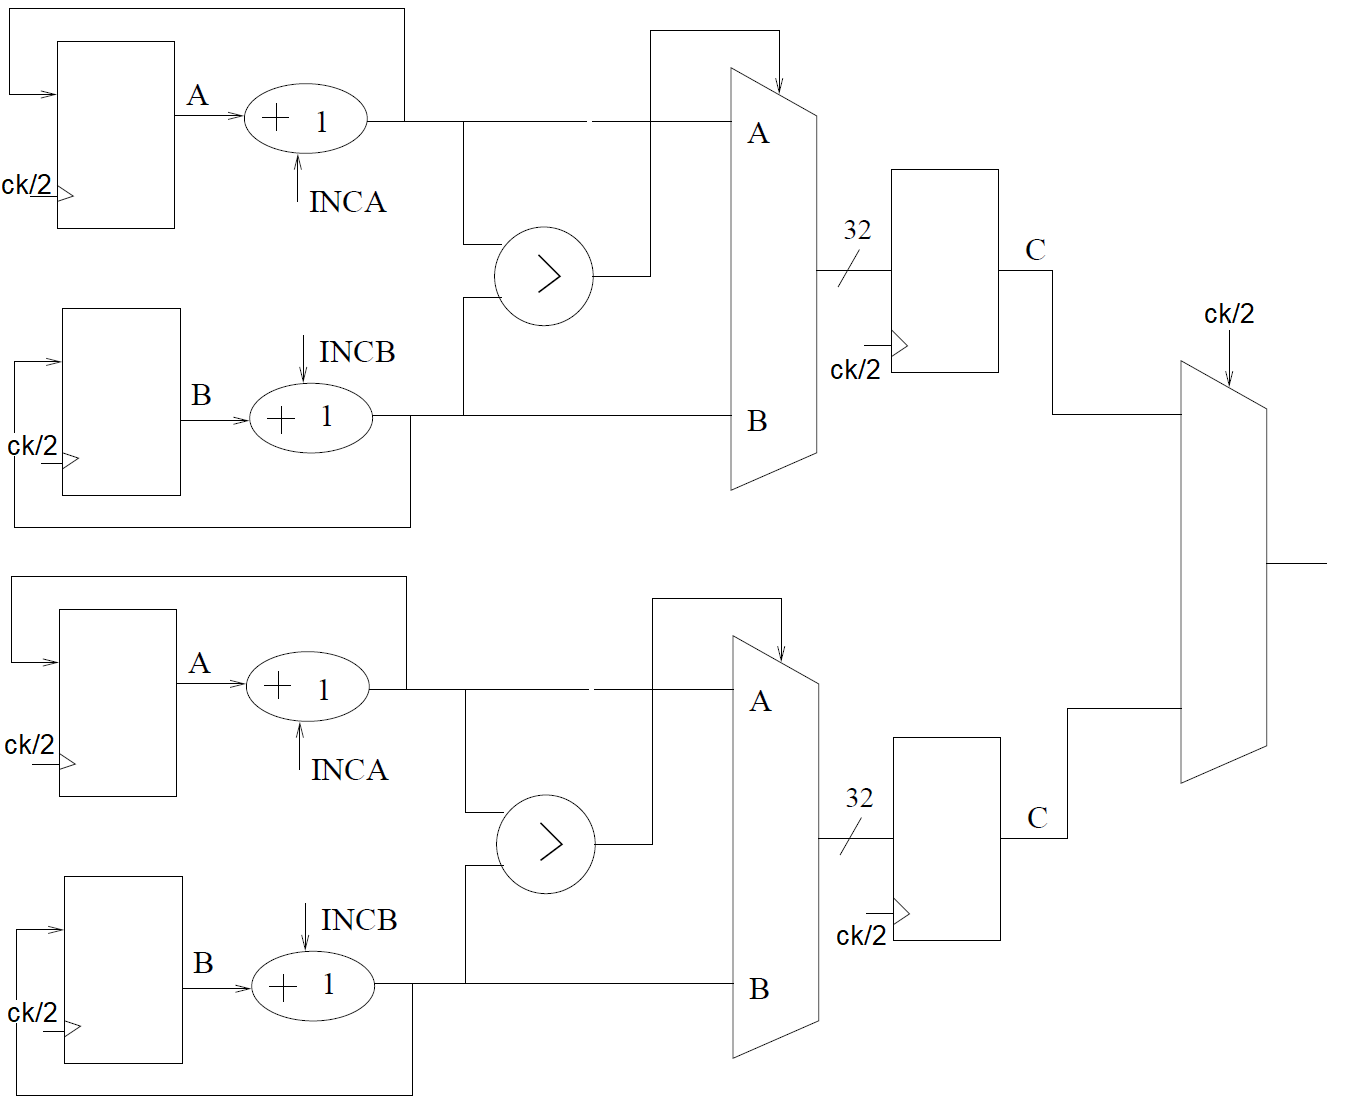
\includegraphics[scale=0.8]{immagini/circuito_parallel}
	\caption{\textit{Configurazione datapath con parallelizzazione a due livelli}}
	\label{circuito_parallel}
\end{figure}
\\
I due datapath lavorano dunque in parallelo, campionando uno sul fronte di salita del clock e l'altro sul fronte di discesa. Di conseguenza la frequenza operativa diventa ora esattamente la metà del caso precedente, dunque $f_{CK}=3.5211 MHz$ a cui corrisponde un periodo di clock pari a $T_{CK}=284 ns$. Ovviamente, nonostante la parallelizzazione, il percorso critico del circuito rimane pari a 140 ns e dunque si può pensare di allungarlo fino al valore del periodo del $T_{CK}$ in modo da poter scalare la tensione di alimentazione $V_{DD}$.\\
Per il calcolo del nuovo valore di alimentazione, vengono fornite delle formule che legano il periodo di clock alla tensione di alimentazione normalizzata rispetto a quella nominale (contrassegnata dalla variabile $u$). Si riportano in seguito i calcoli sviluppati per ottenere la nuova tensione di alimentazione normalizzata:
\begin{center}
	$T(u)=T(V_{DD}=V_{DD, NORM})\frac{0.75u}{u-0.25}=284 ns \Longrightarrow$
\end{center}
\begin{center}
		$\Longrightarrow u=\frac{0.25T(u)}{T(u)-0.75T(V_{DD}=V_{DD,NORM})}\Longrightarrow$
\end{center}
\begin{center}
	$\Longrightarrow u=\frac{0.25\times 284}{284-0.75 \times 142}=0.4$
\end{center}
Ottenuto il valore $u=0.4$, si può ricavare la potenza dissipata da ogni componente tramite l'equazione:
\begin{center}
   $P(V_{DD,new})=P(V_{DD, NOM})\times u^{2}$
\end{center}
Dove per ottenere ottenere i valori di $P(V_{DD, NOM}$ alla frequenza desiderata, ossia $f_{CK}=3.5211 MHz$, si sfrutta la linearità tra potenza e frequenza.
\begin{center}
	$P(V_{DD, NOM})=P(@V_ {DD}=1 V, f_{CK}=5MHz)\times \frac{3.5211 MHz}{5MHz}$
\end{center}
Si riportano nella Tabella \ref{Tab33_3} i nuovi valori di potenza per ogni singolo blocco.\\
\begin{table}[!h]\footnotesize
	\centering
	\begin{tabular}{|c|c|}
		\hline
		\textbf{Cell Type} & \textbf{$P(V_{DD, new})$} \\
		\hline
		\textit{REGISTER} & $0.4225 \mu W \times 0.4^{2}=0.0676 \mu W$\\
		\textit{INCREMENT} & $1.7958 \mu W \times 0.4^{2}=0.2873 \mu W$\\
		\textit{COMPARATOR} & $1.5211 \mu W \times 0.4^{2}=0.2534 \mu W$\\
		\textit{MUX} &$1.1760 \mu W \times 0.4^{2}=0.1882 \mu W$\\
		\hline
	\end{tabular}
	\caption{\textit{Risultati datapath "originale"}}
	\label{Tab33_3}
\end{table}
\\
Nella Tabella \ref{Tab33_4}, sono riportati ora i risultati riferiti alla parallelizzazione del circuito.
\begin{table}[!h]\footnotesize
	\centering
	\begin{tabular}{|c|c|}
		\hline
		\textbf{Parallel Solution} & \\
		\hline
		Delay (critical path) & 284 ns\\
		Allowed Clock Frequency & 3.5211 MHz\\
		Power & $2.6262\mu W$\\
		Area & $3611 \mu m^{2}$\\
		\hline
	\end{tabular}
	\caption{\textit{Risultati datapath "parallelizzato"}}
	\label{Tab33_4}
\end{table}\\
Si può notare che tramite la tecnica della parallelizzazione si ottiene un risparmio dell'$82\%$ rispetto al caso originale, mentre l'area risulta all'incirca raddoppiata.
\\
Si prova ora ad applicare allo stesso modo la tecnica del pipelining che consiste nello spezzare i percorsi combinatori inserendo alcuni registri: in questo modo si riduce drasticamente il percorso critico. \\
Il nuovo circuito è rappresentato in Figura \ref{circuito_pipe}.
\begin{figure}[!htb]
	\centering
	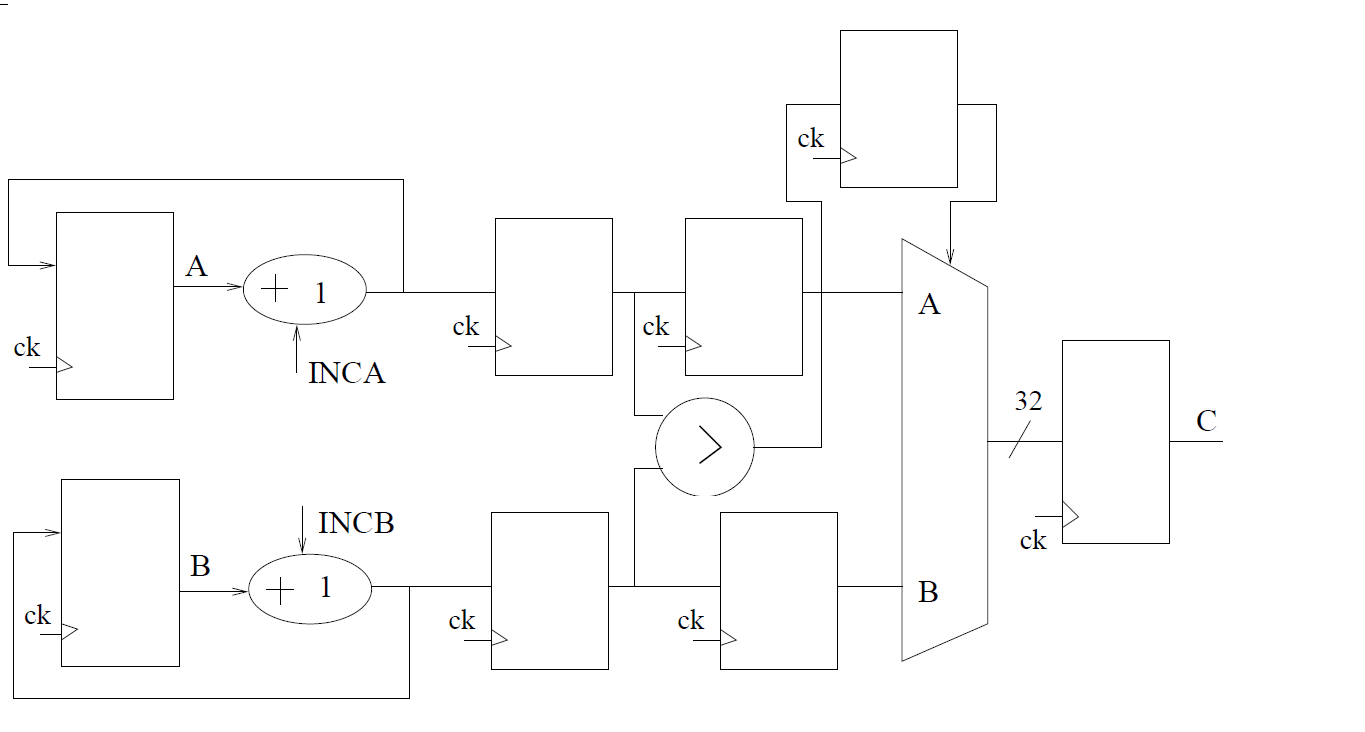
\includegraphics[scale=0.8]{immagini/circuito_pipe}
	\caption{\textit{Configurazione datapath pipelining}}
	\label{circuito_pipe}
\end{figure}
\\
Con questa nuova configurazione il percorso critico diventa quello tra il secondo registro e il comparatore.
\begin{center}
	$T_{critico}=T_{CK->Q}+T_{COMP}=2 ns + 84 ns = 86 ns$
\end{center}
Con questo percorso critico si potrebbe arrivare ad una frequenza di clock pari a $f_{CK}=11.6279 MHz$, ma così facendo si otterrebbero miglioramenti solo nell'ambito della velocità di funzionamento del circuito. L'obiettivo è sfruttare il pipelining per ridurre il consumo senza aumentare le prestazioni: di conseguenza si lascia la frequenza pari a $f_{CK}=7.0422 MHz$. \\
In questo modo il percorso critico risulterà comunque pari sempre a $142 ns$ e si potrà scalare la tensione di alimentazione $V_{DD}$. \\ Si eseguono dunque gli stessi calcoli fatti per il caso della parallelizzazione.
\begin{center}
	$T(u)=T(V_{DD}=V_{DD, NORM})\frac{0.75u}{u-0.25}=142 ns \Longrightarrow$
\end{center}
\begin{center}
	$\Longrightarrow u=\frac{0.25T(u)}{T(u)-0.75T(V_{DD}=V_{DD,NORM})}\Longrightarrow$
\end{center}
\begin{center}
	$\Longrightarrow u=\frac{0.25\times 142}{142-0.75 \times 86}=0.4581$
\end{center}
\begin{center}
	$P(V_{DD,new})=P(V_{DD, NOM})\times u^{2}$
\end{center}
\begin{center}
	$P(V_{DD, NOM})=P(@V_ {DD}=1 V, f_{CK}=5 MHz)\times \frac{7.0422 MHz}{5MHz}$
\end{center}

\noindent Tutti i nuovi valori di potenza dissipata dei singoli blocchi vengono riportati nella Tabella \ref{Tab33_5}
\begin{table}[!h]\footnotesize
	\centering
	\begin{tabular}{|c|c|}
		\hline
		\textbf{Cell Type} & \textbf{$P(V_{DD, new})$} \\
		\hline
		\textit{REGISTER} & $0.0448 \mu W \times 0.4581^{2}=0.1773 \mu W$\\
		\textit{INCREMENT} & $3.5910 \mu W \times 0.4581^{2}=0.7536 \mu W$\\
		\textit{COMPARATOR} & $3.0422 \mu W \times 0.4581^{2}=0.6384 \mu W$\\
		\textit{MUX} &$2.3521 \mu W \times 0.4581^{2}=0.4936\mu W$\\
		\hline
	\end{tabular}
	\caption{\textit{Risultati datapath pipelinato}}
	\label{Tab33_5}
\end{table}

Nella Tabella \ref{Tab33_6}, sono riportati ora i risultati riferiti alla tecnica del pipelining applicata al circuito.
\begin{table}[!h]\footnotesize
	\centering
	\begin{tabular}{|c|c|}
		\hline
		\textbf{Parallel Solution} & \\
		\hline
		Delay (critical path) & 142 ns\\
		Allowed Clock Frequency & 7.0411 MHz\\
		Power & $4.0576\mu W$\\
		Area & $3342 \mu m^{2}$\\
		\hline
	\end{tabular}
	\caption{\textit{Risultati datapath "parallelizzato"}}
	\label{Tab33_6}
\end{table}\\
Si può ben notare come, grazie alla tecnica del pipelining si ottiene un risparmio del 73\% rispetto al caso "originale".\\ Confrontando le due tecniche si può notare come ci sia all'incirca un fattore 2 di differenza tra le potenze risultanti che rende più efficace il metodo della parallelizzazione rispetto al metodo del pipelining. Per quanto riguarda l'area occupata, le due tecniche risultano all'incirca equivalenti, in quanto portano ad un raddoppio dell'area rispetto al circuito originale.\\
Si può pensare ora di sfruttare entrambe le tecniche per scalare il percorso critico, facendolo passare da 86 ns a 284 ns in modo da poter ridurre ancora la tensione di alimentazione e di conseguenza la potenza consumata. Il nuovo circuito è rappresentato in Figura \ref{circuito_parallel_pipe}.
\begin{figure}[!htb]
	\centering
	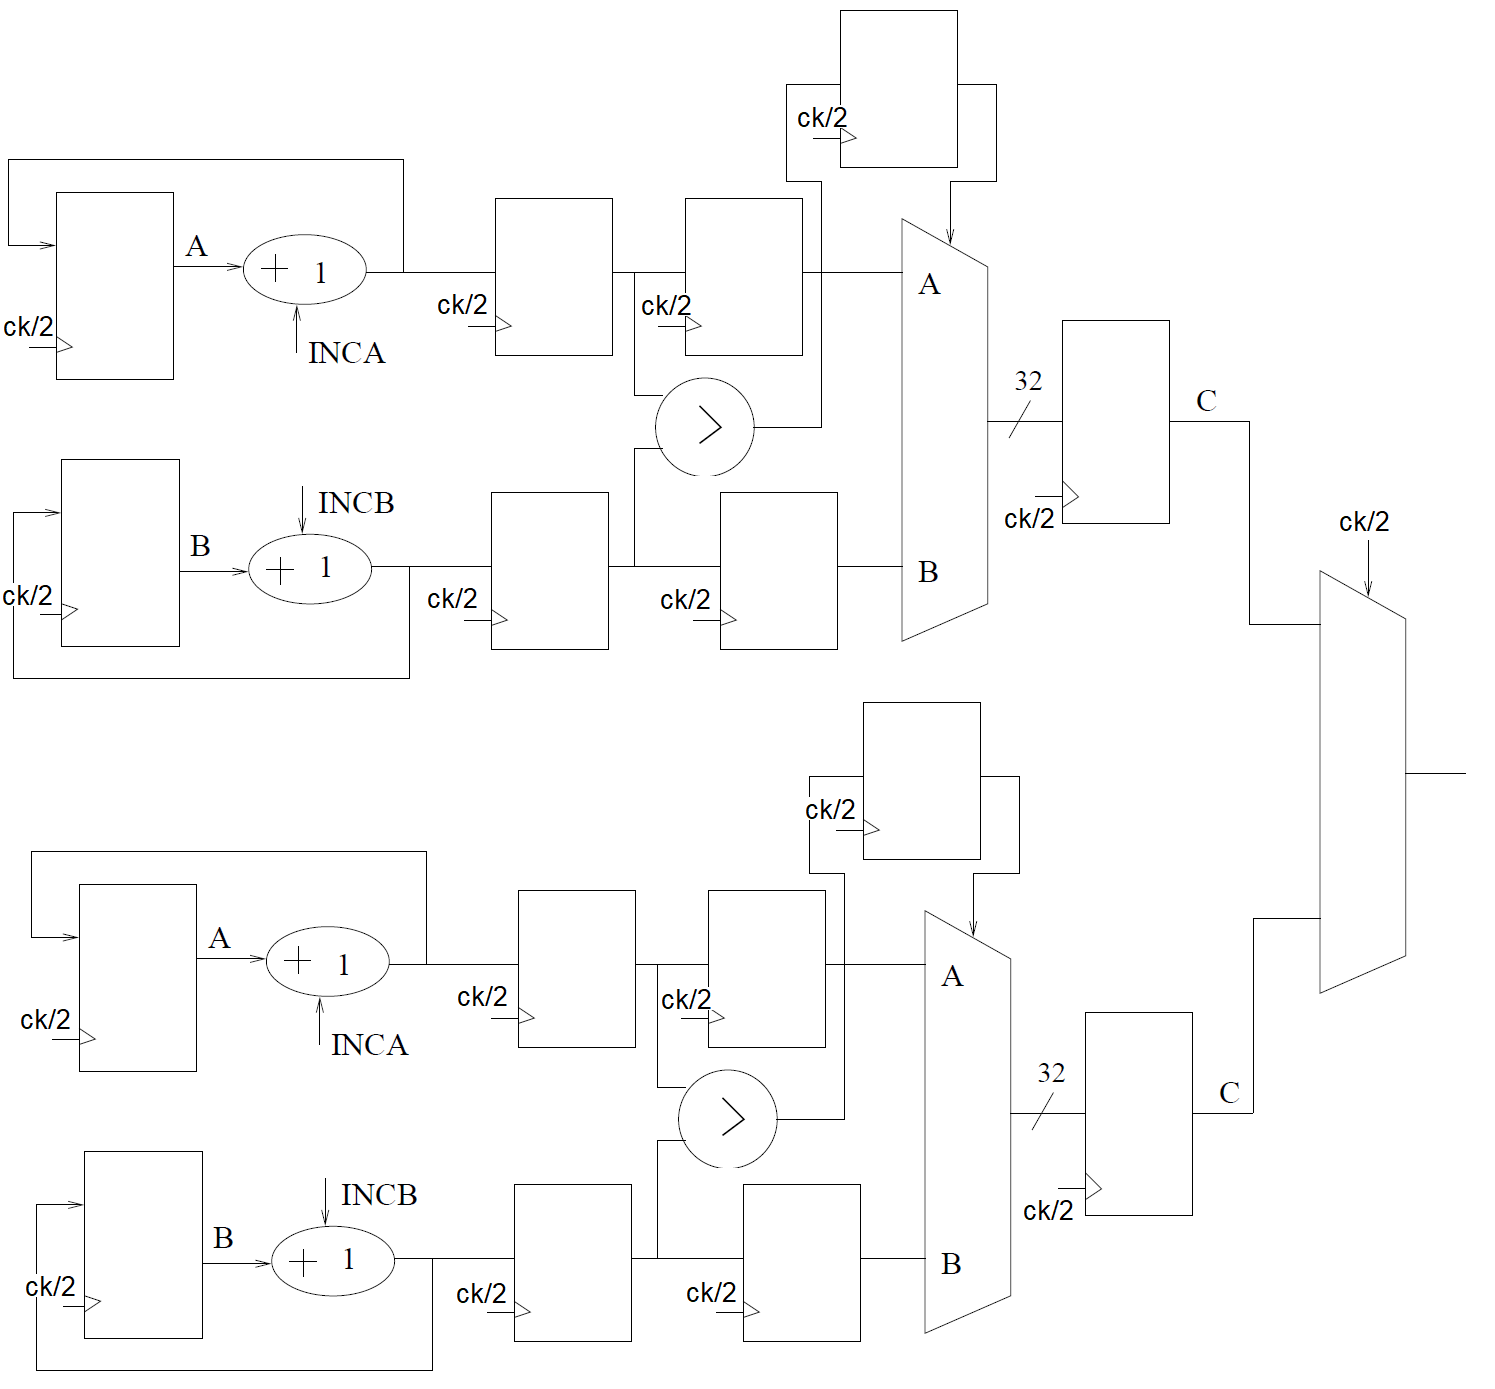
\includegraphics[scale=0.8]{immagini/circuito_parallel_pipe}
	\caption{\textit{Configurazione datapath pipelining}}
	\label{circuito_parallel_pipe}
\end{figure}\\
I risultati di questo nuovo approccio, che vengono calcolati mediante i medesimi passaggi fatti in precedenza sono riportati nella Tabella \ref{Tab33_7}.
\begin{table}[!h]\footnotesize
	\centering
	\begin{tabular}{|c|c|}
		\hline
		\textbf{Parallel and Pipelining Solution} & \\
		\hline
		u &0.3525\\
		Delay (critical path) & 284 ns\\
		Allowed Clock Frequency & 3.5211 MHz\\
		Power & $2.2\mu W$\\
		Area & $7120 \mu m^{2}$\\
		\hline
	\end{tabular}
	\caption{\textit{Risultati datapath "parallelizzato e pipelinato"}}
	\label{Tab33_7}
\end{table}\\
Tuttavia si può notare come questa soluzione non sia ottimale, poiché si ottiene un risparmio di potenza all'incirca pari al caso "parallelizato", ma impiegando un'area due volte superiore.\\
Infine si è analizzato il caso in cui si parallelizzi il sistema a tre livelli, andando a lavorare su una frequenza pari a $f_{ck}/3$: si scala di conseguenza il percorso critico, portandolo a 426 ns e si può ridurre ulteriormente la tensione di alimentazione $V_{DD}$. Anche in questo caso si riportano esclusivamente i risultati dei calcoli in Tabella \ref{Tab33_8}. 
\begin{table}[!h]\footnotesize
	\centering
	\begin{tabular}{|c|c|}
		\hline
		\textbf{Parallel and Pipelining Solution} & \\
		\hline
		u &0.3333\\
		Delay (critical path) & 426 ns\\
		Allowed Clock Frequency & 2.347 MHz\\
		Power & $1.76596\mu W$\\
		Area & $5358 \mu m^{2}$\\
		\hline
	\end{tabular}
	\caption{\textit{Risultati datapath "parallelizzazione a tre livelli"}}
	\label{Tab33_8}
\end{table}\\
Si può concludere affermando che la soluzione che porti al minor consumo di potenza sia la parallelizzazione a tre livelli, che comporta una riduzione della potenza pari a circa 8 volte la potenza del caso "originale". L'unico svantaggio di questa soluzione è che comporta un'area tre volte superiore.\\
Se si vuole cercare un trade-off tra area e potenza, sicuramente la soluzione migliore è la parallelizzazione a due livelli, che comporta un risparmio di potenza di circa 6 volte rispetto al caso originario, utilizzando "solo" un'area due volte superiore.\\
\subsection{Are you sure it was correct?}
Nelle Figura \ref{Timing3_1} e \ref{Timing3_2}, sono riportati i timing diagram rispettivamente del circuito originale e del caso "parallelizzato".
\begin{figure}[!htb]
	\centering
	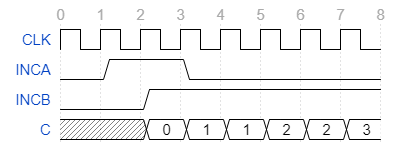
\includegraphics[scale=2]{immagini/3_timing2}
	\caption{\textit{Timing datapath "originale"}}
	\label{Timing3_1}
\end{figure}\\
\begin{figure}[!htb]
	\centering
	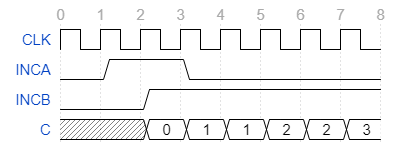
\includegraphics[scale=2]{immagini/3_timing2}
	\caption{\textit{Timing datapath "parallelizzato"}}
	\label{Timing3_2}
\end{figure}\\
Si può ben notare come l'uscita del datapath nel secondo caso non sia corretta. Questo errore è dovuto al fatto che nel circuito siano presenti dei loop: questo implica che l'elaborazione del dato $i+1-esima$ può dipendere dall'elaborazione $i-esima$ e dunque non può essere effettuata su un altro circuito, come nel caso della parallelizzazione.





